
% Falar do problema
% O que vai fazer neste capitulo
% 

The development of par-gem5 \cite{pargem5} solved one problem of Gem5 \cite{TheGem5Simulator}, which is the low performance even with a power full host machine. As exhibited in the \autoref{subsec:pargem5}, the accuracy is no longer perfect, and a trade-off between these occurs. Concerning the current works on this subject, none of them fulfilled the three characteristics presented in the \autoref{tab_OverviewDynamicQuantum}, therefore they can not be employed in the par-gem5. 

To overcome these limitations and find the optimal quantum automatically, there were developed some algorithms in the scope of this dissertation, and in this chapter, they will be described and explained in detail. These algorithms are called: ADALINE, increment, \glsxtrfull{pc}, and repetition. As the name suggests, the first one is based on the ADALINE \gls{nn}. The following is used by the previous to dynamically adapt the increment value. \gls{pc} algorithm analyses the executed instructions to identify if their execution may result in inaccuracy. These two provide support for the remaining ones, meaning they cannot function independently. The last one tries to identify loops within the execution of the simulation to accordingly adapt the quantum.  

\begin{figure}[H]
	\centering
 	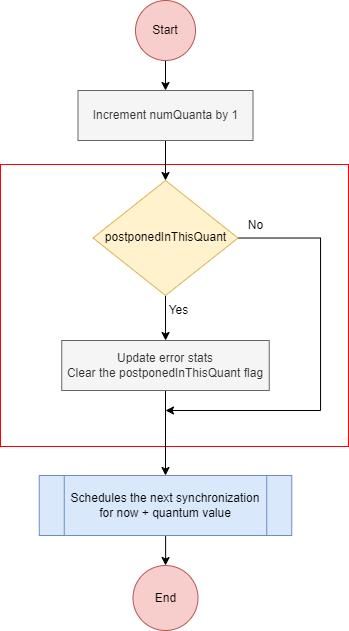
\includegraphics[width=0.5\linewidth]{Images/GlobalSyncEventStatic.png}
 	\caption{Quantum definition in the synchronization process}
	 \label{fig_GlobalSyncEventStatic}
\end{figure}

In the current state of par-gem5, the quantum attribution is done as presented in the latter image. The simulator enters a synchronization state that establishes whether the simulation should continue or not. If affirmative, the next synchronization is scheduled for the current time plus the pre-defined quantum. If not, it finishes the workload. The red rectangle defines the zone where the adaptive quantum should be implemented, in a way that the schedule function will use, for the next synchronization event, the quantum resulting from the algorithm. 

\section{Benchmarks}

When an engineer designs an \gls{asic}, for example, in the end he needs to verify if the project meets the requirements. Therefore, the engineer needs to execute tests that are called benchmarks. They are designed to measure the performance, capabilities, or efficiency of a system, component, or software application. There are different types of benchmarks, each one emphasizing an area of interest. \gls{cpu}, network, and storage are some examples. 

In the context of this dissertation, it will be used two \gls{cpu} benchmarks, the bare-metal bubble sort and the \gls{npb}. The host and the target systems have the configurations present in the \autoref{tab:hostSystemConfig} and \autoref{tab:targetSystemConfig} respectively.   

\begin{table}[!htb]
    \caption{System Configurations}
    \begin{minipage}{.5\linewidth}
      \centering
      \subcaption{Host}
        \resizebox{\textwidth}{!}{%
        \begin{tabular}{lll}
        \cline{1-2}
        \multicolumn{1}{|l|}{CPU} & \multicolumn{1}{l|}{AMD Ryzen 3990x (64 cores, 128 threads)} &  \\ \cline{1-2}
        \multicolumn{1}{|l|}{RAM} & \multicolumn{1}{l|}{128GB of 3200MHz DDR4-DRAM} &  \\ \cline{1-2}
        \multicolumn{1}{|l|}{OS} & \multicolumn{1}{l|}{Ubuntu Linux 20.04} &  \\ \cline{1-2}
         &  & 
        \end{tabular}%
        }
        \label{tab:hostSystemConfig}
    \end{minipage}%
    \begin{minipage}{.5\linewidth}
        \centering
        \subcaption{Target}
        \resizebox{\textwidth}{!}{%
            \begin{tabular}{lll}
            \cline{1-2}
            \multicolumn{1}{|l|}{CPU} & \multicolumn{1}{l|}{ARM64, AtomicSimpleCPU @ 2GHz} &  \\ \cline{1-2}
            \multicolumn{1}{|l|}{Caches} & \multicolumn{1}{l|}{64kiB L1-D, 32kiB L1-I, 2MiB L2 shared} &  \\ \cline{1-2}
            \multicolumn{1}{|l|}{Main Memory} & \multicolumn{1}{l|}{DDR3 RAM @ 1600MHz} &  \\ \cline{1-2}
            \multicolumn{1}{|l|}{Periph. Sub-system} & \multicolumn{1}{l|}{Real View Virtual Express V1} &  \\ \cline{1-2}
             &  & 
            \end{tabular}%
        }   
        \label{tab:targetSystemConfig}
    \end{minipage} 
\end{table}

\subsection{Bare-metal Bubble Sort}

The main objective of this benchmark, as implied by its name, is to rearrange an array in such a way that elements with higher values are positioned at the top. The algorithm employed for this task is quite straightforward. It involves a loop that iterates through the input list, examining each element in turn. During each iteration, the algorithm compares the current element with the one that follows it and, if necessary, swaps their values. This process continues until the entire array is sorted according to the desired criterion. It was designed to attain a near best-case simulation throughput, meaning that thread synchronizations and accesses to shared memory are reduced to a minimum.

\begin{figure}[H]
	\centering
 	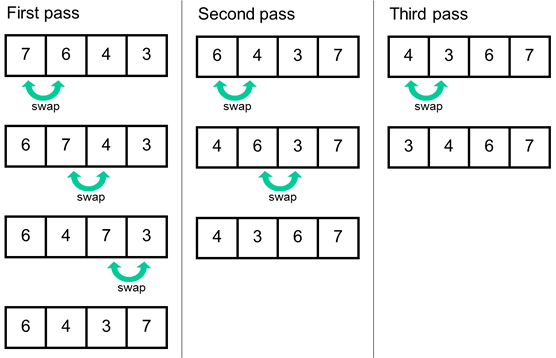
\includegraphics[width=0.7\linewidth]{Images/bubble_sort.png}
 	\caption{Bubble sort example}
	 \label{fig_bubble_sort}
\end{figure}

This benchmark operates in a bare-metal environment, which means it is implemented without the use of an operating system (OS). In a bare-metal setup, the program runs directly on the hardware without the mediation or assistance of an operating system. This approach is often chosen for performance-critical or resource-constrained applications where direct control over the hardware is necessary, and there is no need for the additional services and abstractions provided by an operating system.

\subsection{NPB}

The \glsxtrfull{npb} \cite{bailey1994parallel} is a group of a small set of programs designed to help the performance evaluation of parallel supercomputers. In total, there are eight benchmark specifications, five kernels, and three pseudo-applications. The kernel benchmarks are:

\begin{itemize}
    \item \textbf{Integer Sort (IS):} Performs a sort operation where both integer computation speed and communication performance are tested.

    \item \textbf{Fast Fourier Transform (FT):} Solves a three-dimensional partial differential equation using \glsxtrfullpl{fft}. Long-distance communication performance is the main evaluation point. 

    \item \textbf{MultiGrid (MG):} It is a simplified multigrid kernel that requires highly structured long-distance communication, thus short and long-distance data communication are evaluated.

    \item \textbf{Conjugate Gradient (CG):} Computes an approximation to
    the smallest eigenvalue of a large, sparse, symmetric positive definite matrix. The main goal is to test irregular long-distance communication.

    \item \textbf{Embarrassingly Parallel (EP):} It provides an estimate of the
    upper achievable limits for floating point performance, with no significant inter-process communications.
\end{itemize}

The pseudo-applications are the \textbf{Block Tridiagonal (BT)}, \textbf{Scalar Pentadiagonal (SP)}, and \textbf{Lower-Upper symmetric Gauss-Seidel(LU)} benchmarks. Each of these benchmarks is designed to solve a synthetic system of nonlinear partial differential equations using a distinct algorithm. The names of the benchmarks correspond to the specific algorithms employed in solving these mathematical problems.

Moreover, \gls{npb} implemented benchmark classes, that is, the problem size of each workload can be modified. There were implemented 8 problem sizes (S, W, A, B, C, D, E, and F), where S is the smaller one and F is the bigger one. In the context of this dissertation, only the W size will be considered.

\section{ADALINE}

Adaptive filters are commonly used for the reason that they possess the ability to automatically adjust their own parameters and their design necessitates minimal or no prior knowledge of signal \cite{haykin1996linear}. One application of this filters can be in the development of a \glsxtrfull{anc} algorithm. A generic scheme can be found in the image bellow.

\begin{figure}[H]
	\centering
 	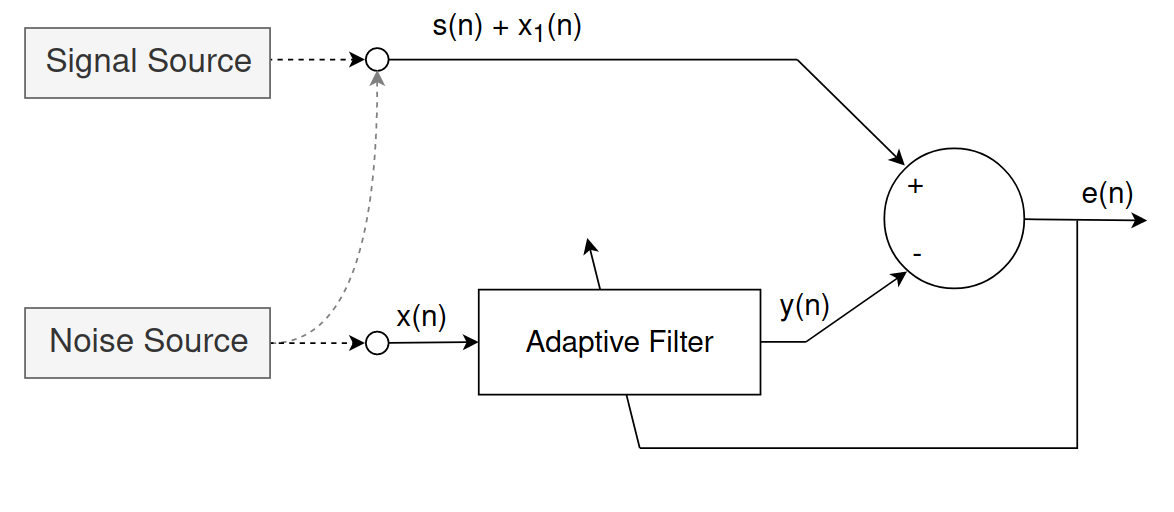
\includegraphics[width=0.7\linewidth]{Images/AdaptiveNoiseCancellationScheme.png}
 	\caption{\gls{anc} scheme}
	 \label{fig_AdaptiveNoiseCancellationScheme}
\end{figure}

$S(n)$ is the input that has the signal mixed with the noise, and $X(n)$ receives only the noise, hence it is a noise reference. If the noise in $S(n)$ was the same as the one presented in $X(n)$, it would only be needed to subtract the $X(n)$ to $S(n)$, nevertheless this noise is different because it is attenuated, delayed, and filtered by noise path. For these reasons, an adaptive filter should be utilized, allowing $Y(n)$ to closely resemble $X_{1}(n)$. $E(n)$ will be the output without the error. It is also used by the filter in order to adapt their weights.

A comparison can be made to the par-gem5 world. The signal is the quantum, the noise is the simulation error, and the output is the quantum without the error. Also, the $X_{1}(n)$ and $X(n)$ are different due to the impossibility of calculate exactly $X_{1}(n)$ in runtime. When a benchmark is running, the simulation error obtained is refereed to the worst case scenario. In other words, the simulator analyses when there is a cross-schedule event, and the time difference between when that happens and the next synchronization is considered the error, since it considers that event must be postponed. However, most of the times it is not true, and the event is not postponed, causing a smaller error. To accurate analyse what was the impact of inaccuracy, to obtain $X_{1}(n)$, it would be needed to run firstly the sequential simulation, killing all the benefits of par-gem5 \cite{pargem5}. The next equation describes how the worst case error estimation is calculated. 

\begin{equation}
    \label{eq_errSim}
    \centering
        \Large
        e_{rel,t} = \frac{t_{sim,meas}}{t_{sim,meas}-\sum_{i=0}^{Q}t_{i,max\_pp}} -1  = \frac{t_{sim,meas}}{t_{sim,est}}-1
        \normalsize
\end{equation}
\vspace{0.3cm}

In each quantum the postpone-mechanism records which event experienced the most significant time shift caused by the postponement, $t_{i,max\_pp}$. $Q$ is the number of simulated quanta and $t_{sim,meas}$ is the measured simulation time. 


\subsection{Adaptive Filter}

Following the \autoref{fig_AdalineSquematic}, the adaptive filter will be responsible for adapting the weights of the ADALINE \gls{nn}. It uses the \autoref{eq_LSM} for the training, where it is essential to carefully choose an appropriate learning rate.

The learning rate is a constant that is chosen at the beginning of the simulation and it is not modified. This parameter compromises a trade-off between control speed and stability. With lower values, the learning process is fast nevertheless, it is likely to become an unstable control system. With higher values, stability is granted, but the learning process is very slow, taking a lot of time to be operational.
Finding the best value is not linear, therefore an iterative approach was used. 

A small simulation was done and in each quantum synchronization, the values of the quantum and the error were recorded. Furthermore, in this test, the quantum was incremented 1 microsecond every time a record was done. Then, the ADALINE algorithm was implemented in Matlab, obtaining the results illustrated on \autoref{fig:learningRateTests}.

\begin{figure}
\centering
\begin{subfigure}{\textwidth}
    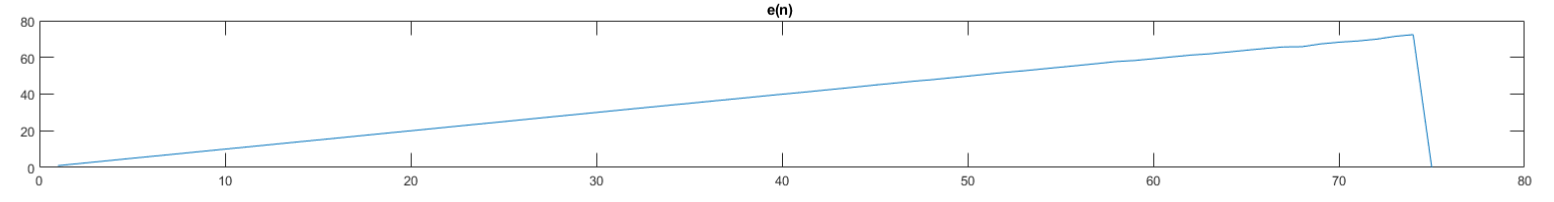
\includegraphics[width=\textwidth]{Images/AF1.png}
    \caption{ $\mu = 1 * 10^{-16} $ }
    \label{fig:AF1}
\end{subfigure}
\begin{subfigure}{\textwidth}
    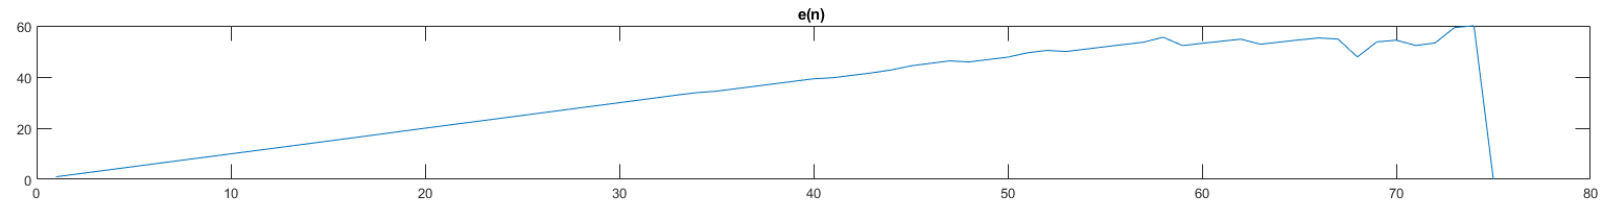
\includegraphics[width=\textwidth]{Images/AF2.png}
    \caption{ $\mu = 1 * 10^{-17}$ }
    \label{fig:AF2}
\end{subfigure}
\begin{subfigure}{\textwidth}
    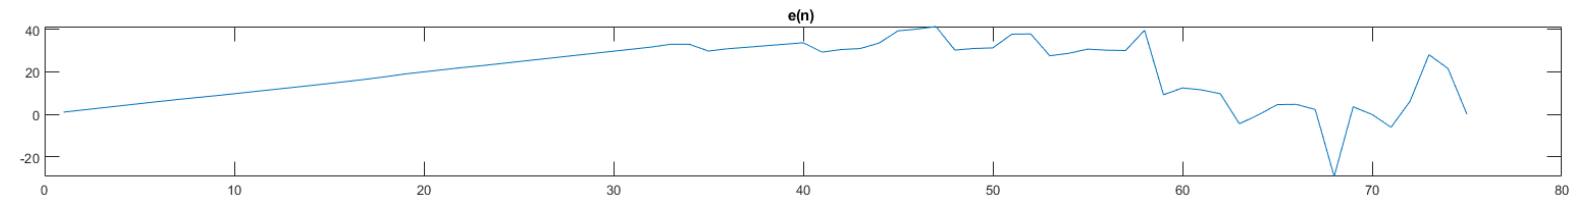
\includegraphics[width=\textwidth]{Images/AF3.png}
    \caption{ $\mu = 1 * 10^{-18}$ }
    \label{fig:AF3}
\end{subfigure}
        
\caption{Control action with different learning rate values}
\label{fig:learningRateTests}
\end{figure}

 The aforementioned mention trade-off can be observed, where for $\mu > 1 * 10^{-16} $, the results were similar to \autoref{fig:AF1}, and for $\mu < 1 * 10^{-18} $, the system become even more unstable. To choose the learning rate, the logarithmic scale is used, as small variations in the $\mu$ do not result in a significant change. From the results was concluded that the best value for $\mu$ is $1 * 10^{-17}$. 

Although on this test when $\mu$ was equal to $1 * 10^{-17}$ did not result in an unstable control system, there is a possibility that it could happen, for example, when there are huge error variations. Typically, these variations occur when the synchronization time is much longer than the ideal case, which requires to reset the algorithm. Regarding the results on \cite{pargem5}, where it was observed the inaccuracy grows with increasing quantum and number of cores, it was also implemented a \textit{safeQuanta}, a value that is smaller than the actual quantum. It depends on the previously mentioned characteristics, hence it can adapt to the present situation. The next flowchart illustrates how the reset system works.

\begin{figure}[H]
	\centering
 	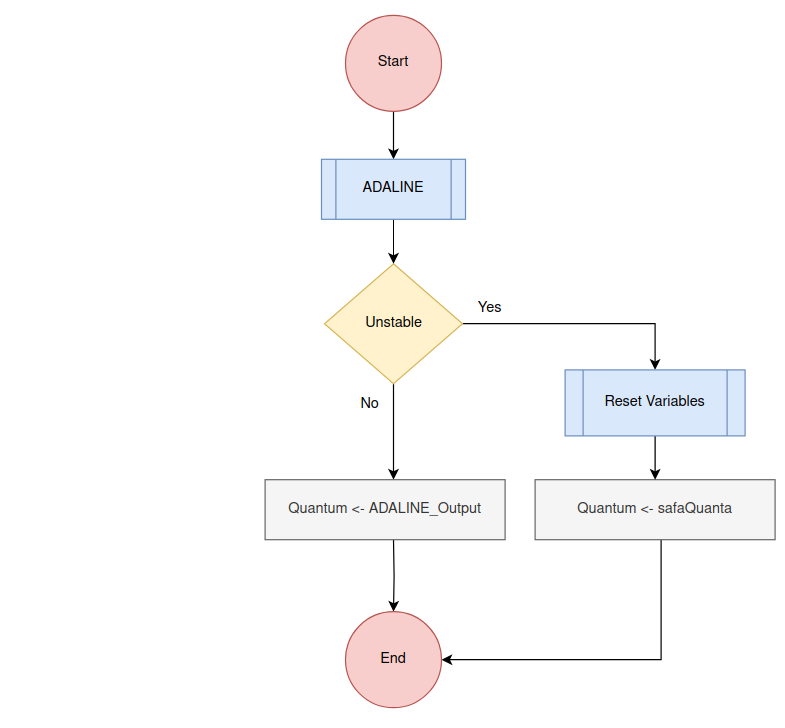
\includegraphics[width=0.5\linewidth]{Images/ResetSystemADALINE.png}
 	\caption{Reset system in ADALINE algorithm}
	 \label{fig_ResetSystemADALINE}
\end{figure}

If the ADALINE output is negative, means it becomes unstable, and needs a reset. In the reset, all the variables used in the calculation are set into their initial conditions, sacrificing simulation performance. For this reason, it is desirable to have the least resets possible.

\subsection{TDL}

As the simulation precedes, there is more data to analyse, taking away performance from the \gls{nn}. Stella et al. \cite{noiseCancelingADALINE} presented one example of an application where this problem is also present. The solution to make full use of the ADALINE network as an adaptive filter was the implementation of a \glsxtrfull{tdl}. Its operating method is described in the figure below. 

\begin{figure}[H]
	\centering
 	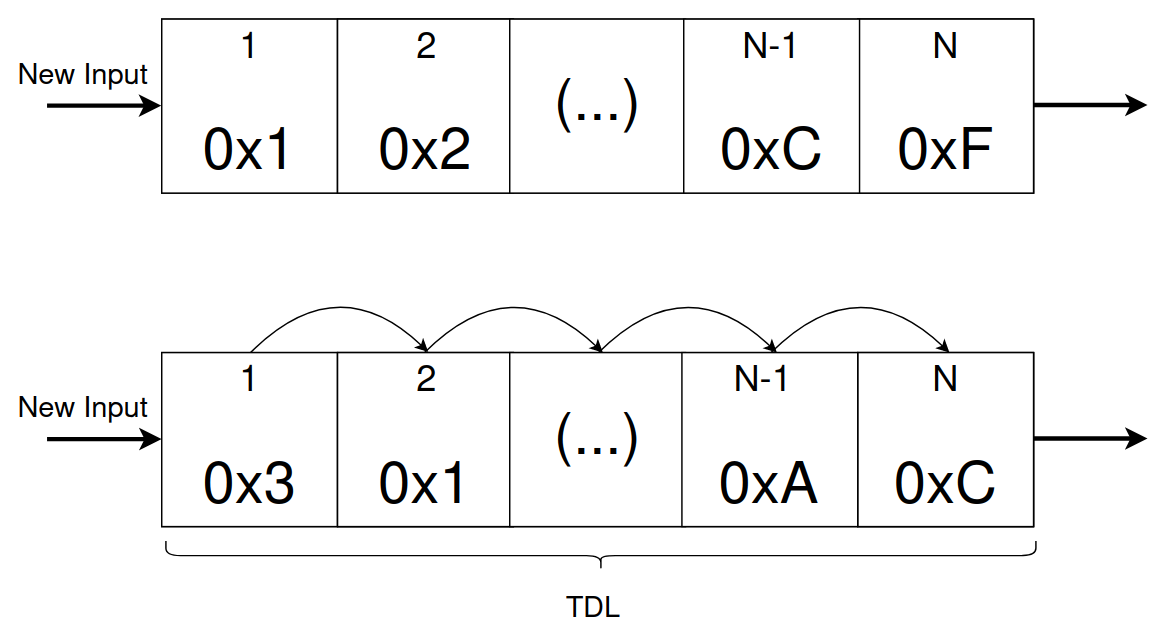
\includegraphics[width=0.5\linewidth]{Images/TDL.png}
 	\caption{\gls{tdl} working method}
	 \label{fig_TDL}
\end{figure}

One input is considered $N$ times, being $N$ the size of the \gls{tdl}. When a new input arrives, the oldest one is discarded. In the end, the \gls{tdl} have always the signal at the current time, the previous input signal, and so on. Combining the \gls{tdl} with the ADALINE, efficiency, and performance are no longer sacrificed. This approach was implemented in the noise source since it receives new data in each new quantum evaluation. 

\gls{tdl} size varies from application to application. In this case, when the size is small, the learning process may be subpar, but it also becomes less sensitive to variations in the noise. Conversely, a larger size leads to more effective weight adjustments through improved learning, but it makes the \gls{nn} more susceptible to noise variations. To choose the best size for this scenario, a small test was done. The results are presented in the following graph.

\begin{figure}[H]
	\centering
 	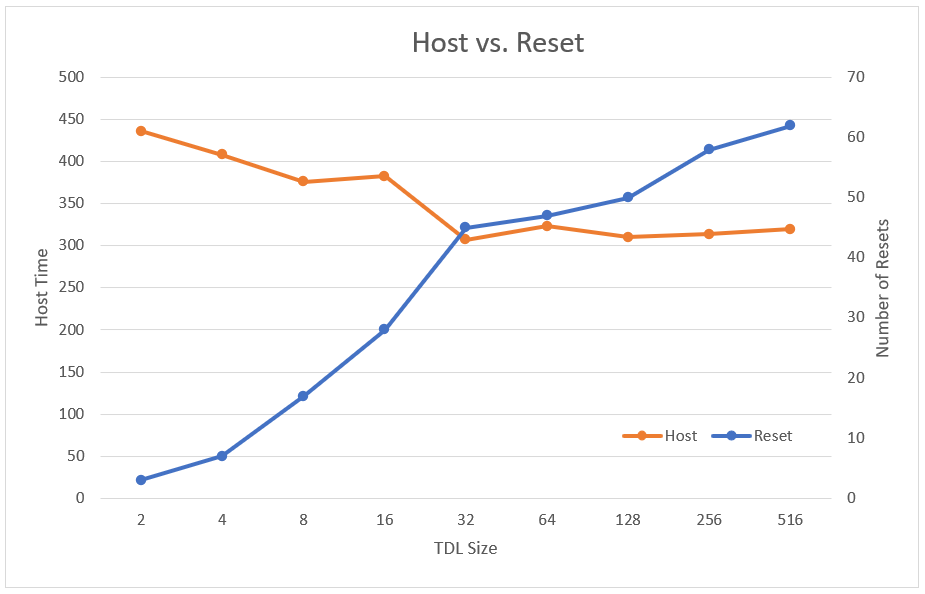
\includegraphics[width=0.7\linewidth]{Images/ResetVsHost.png}
 	\caption{Reset vs. Host}
	 \label{fig_ResetVsHost}
\end{figure}

To have maximum performance on the simulator, only base $2^{n}$ sizes were chosen, where $n \in N$. Observing the outcome, it can be seen that there is a point where the host time does not improve significantly, however the number of resets continues increasing. Each reset has a performance impact, as it requires resetting every variable to their initial conditions. Therefore, it is desirable to minimize the number of resets whenever possible. In the end, it can be concluded that the best size to be used is 32, and for this reason it was used for the subsequent tests.

\subsection{Quantum Increment}

The ADALINE's algorithm output, that is, the filtered quantum, will be always lower than source. Using this new quantum implies that there will be a point in time when it becomes too small, primarily because it fails to exhibit a value increment. This situation inevitably leads to a trade-off, wherein performance is compromised. To strike the optimal balance, it becomes necessary to increment the quantum value. This adjustment should occur when no errors are detected in the system. \autoref{fig_ADALINE_v1} presents the flowchart for the ADALINE algorithm.

\begin{figure}[h!]
	\centering
 	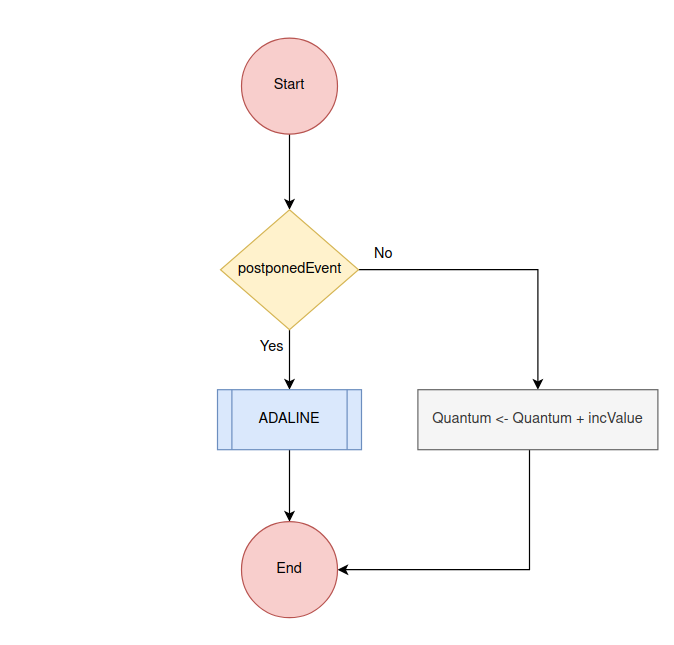
\includegraphics[width=0.5\linewidth]{Images/ADALINE_v1.png}
 	\caption{ADALINE flowchart}
	 \label{fig_ADALINE_v1}
\end{figure}

An error exists when an event must be postponed. Par-gem5 \cite{pargem5} introduces a flag called \textit{postponedInThisQuanta}, that triggers if the previous scenario occurs. When the simulator enters in the synchronization state, this flag is verified to decided if the quantum should be incremented or not. The increment value should have a balance, in the way that with a smaller increment the performance may not be improved, and with a high value the accuracy may be ruined. According to \cite{pargem5}, the quantum of 1 microsecond gives a good trade-off between the those two, thus it was chosen to use a increment 10 times lower. This value enables a significant balance without causing any harm.

\subsection{Results}

The aforementioned benchmarks executed the developed algorithm with different number of cores. The results obtain are depicted in the \autoref{fig:results_ADA}. 

\begin{figure}[]
\centering
\begin{subfigure}{\textwidth}
    \centering
    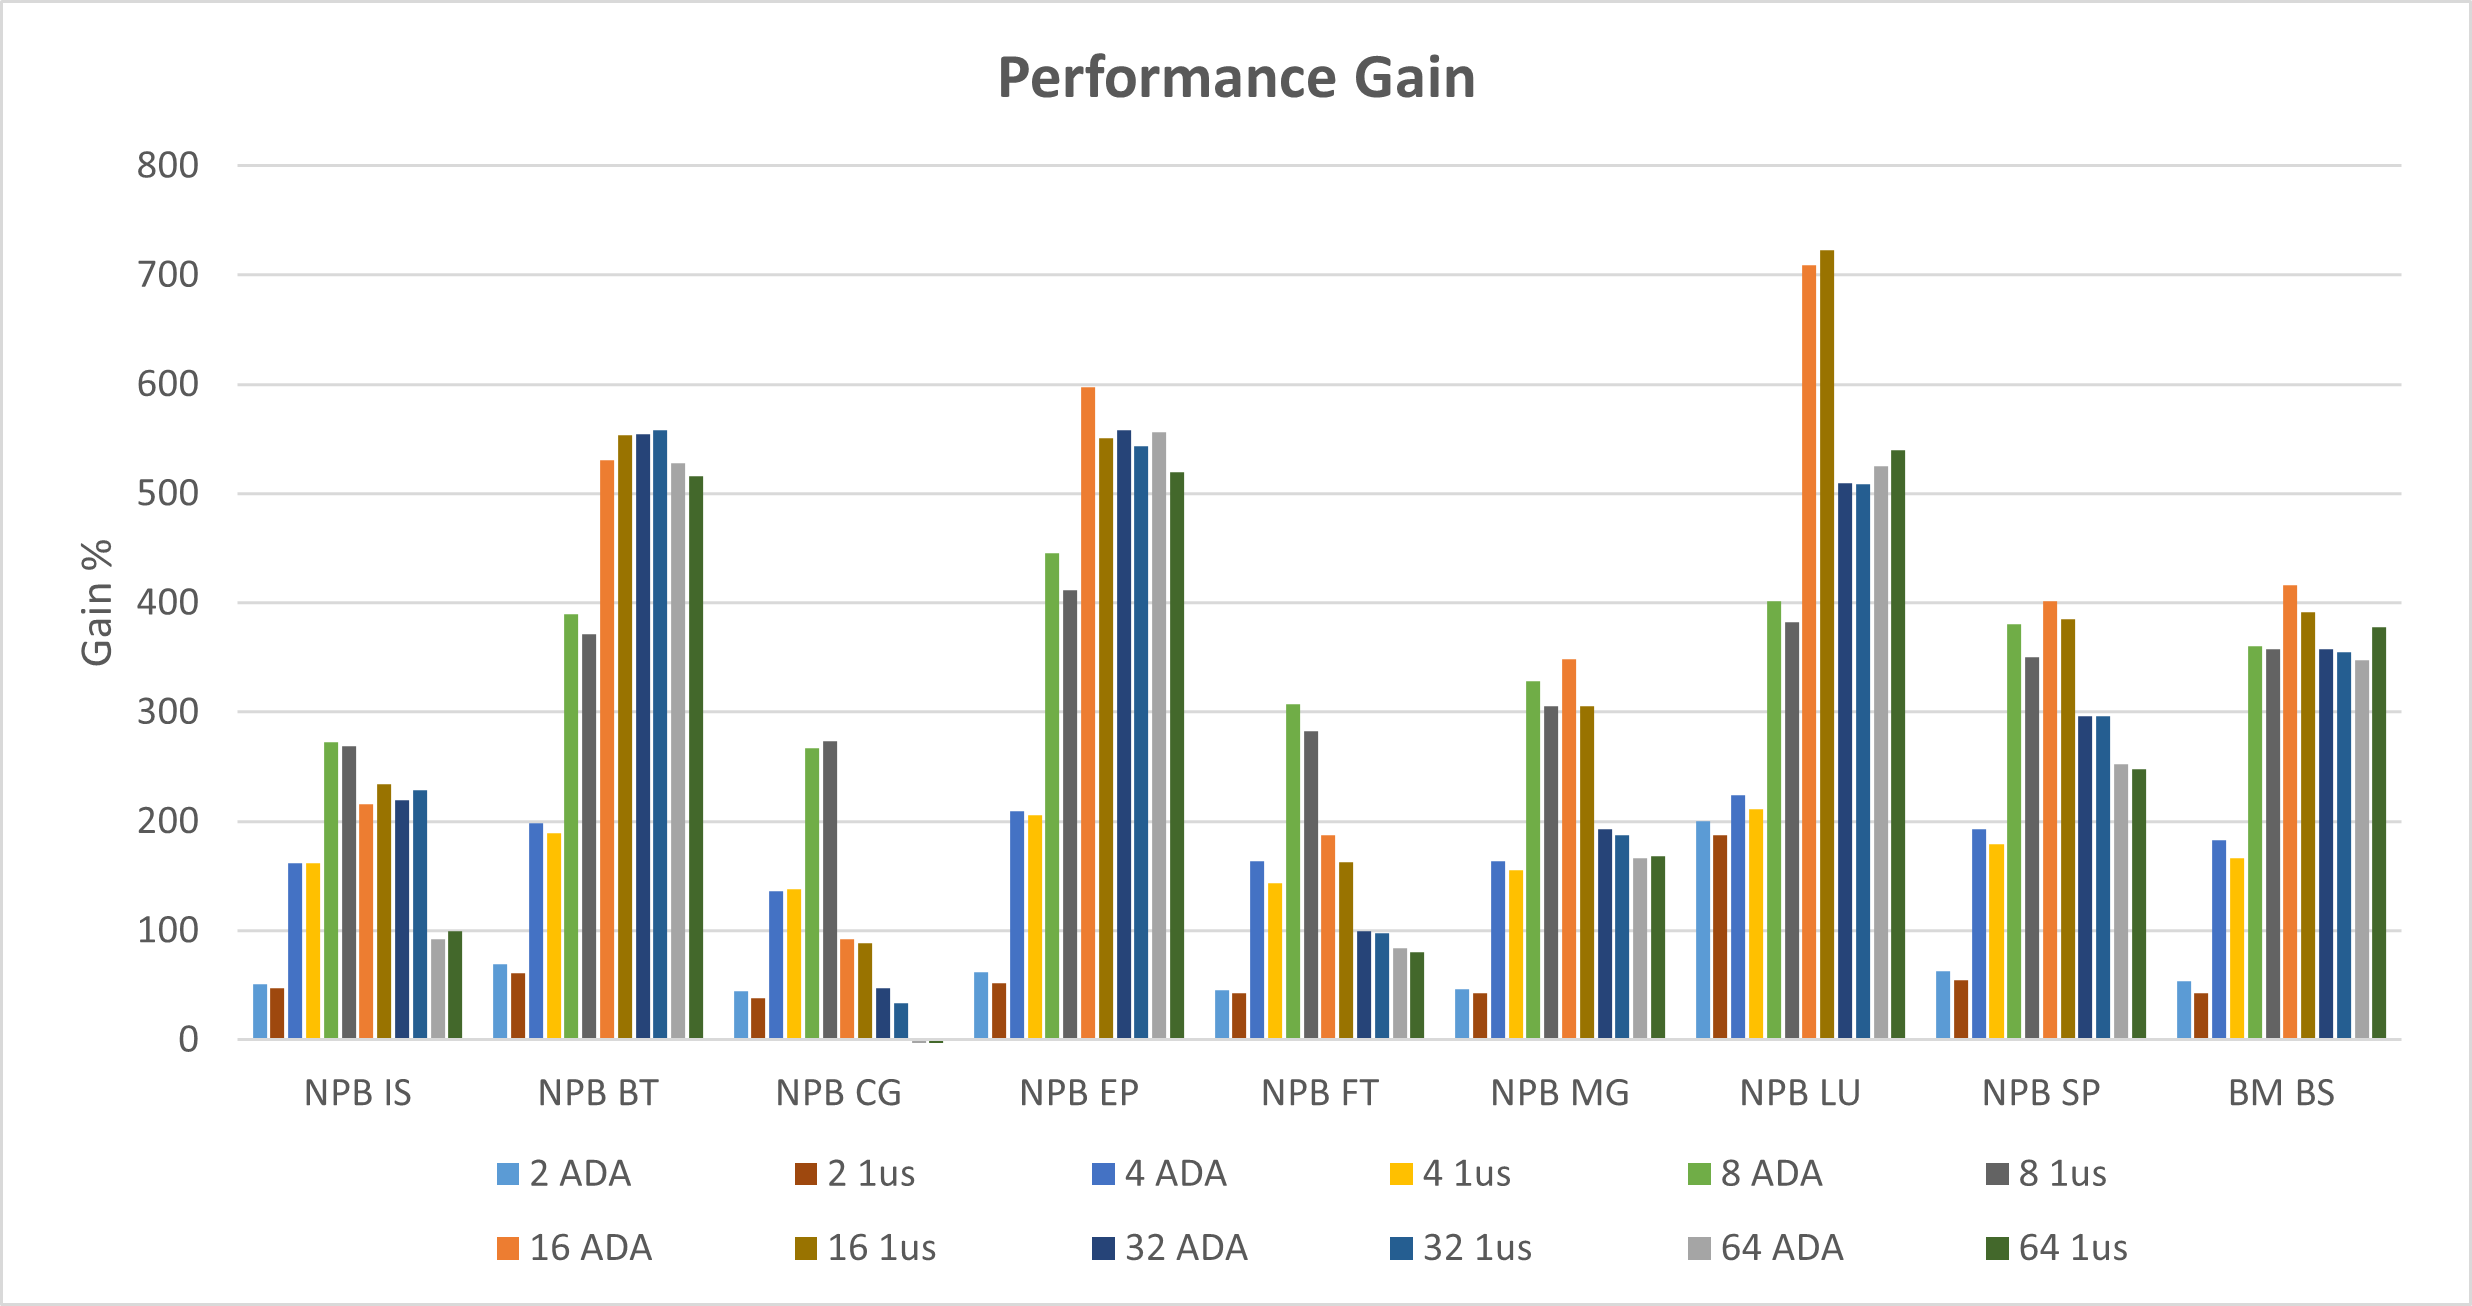
\includegraphics[width=0.75\textwidth]{Images/Performance_ADA.png}
    \caption{ Performance gain}
    \label{fig:Performance_ADA}
\end{subfigure}
\begin{subfigure}{\textwidth}
    \centering
    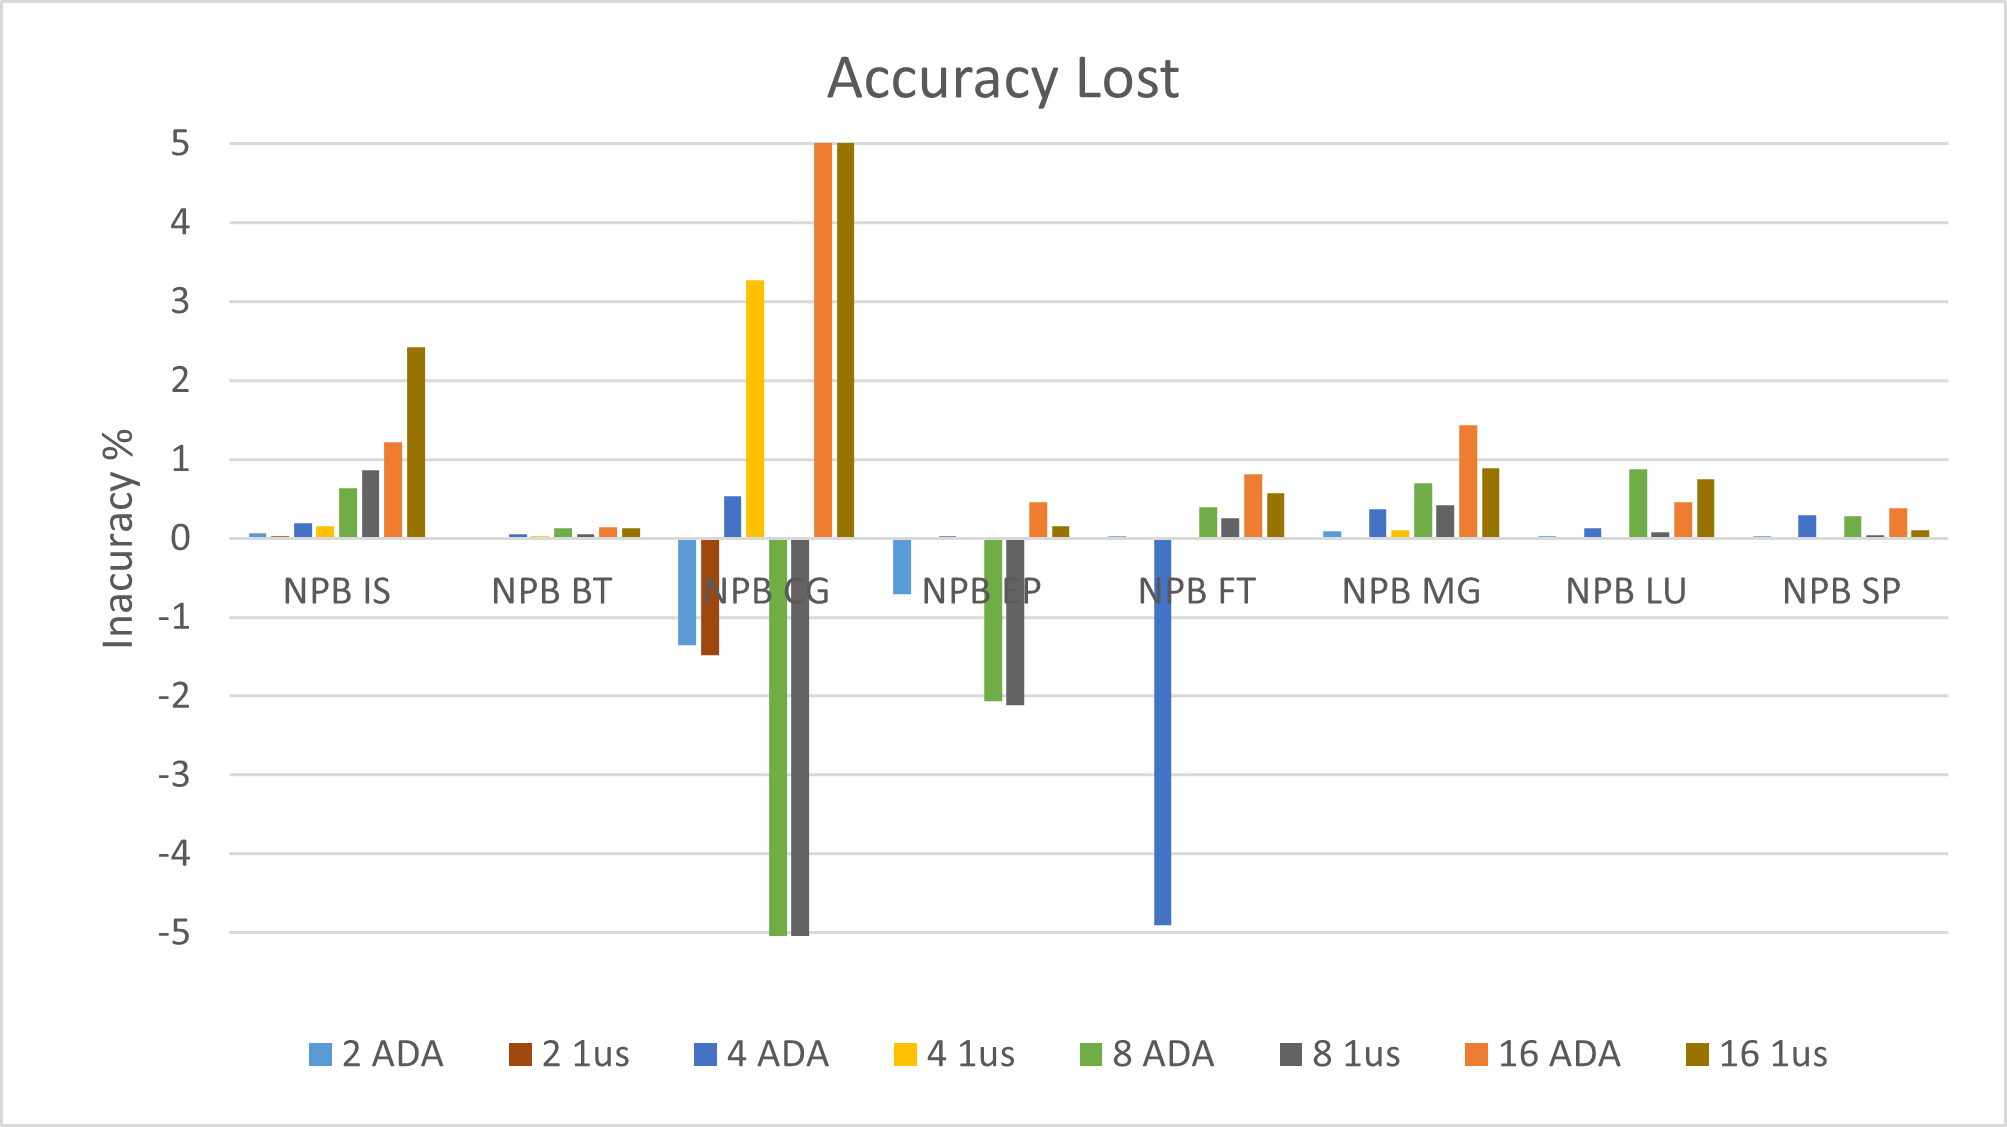
\includegraphics[width=0.75\textwidth]{Images/Accuracy_ADA.png}
    \caption{ Accuracy lost}
    \label{fig:Accuracy_ADA}
\end{subfigure}
\begin{subfigure}{\textwidth}
    \centering
    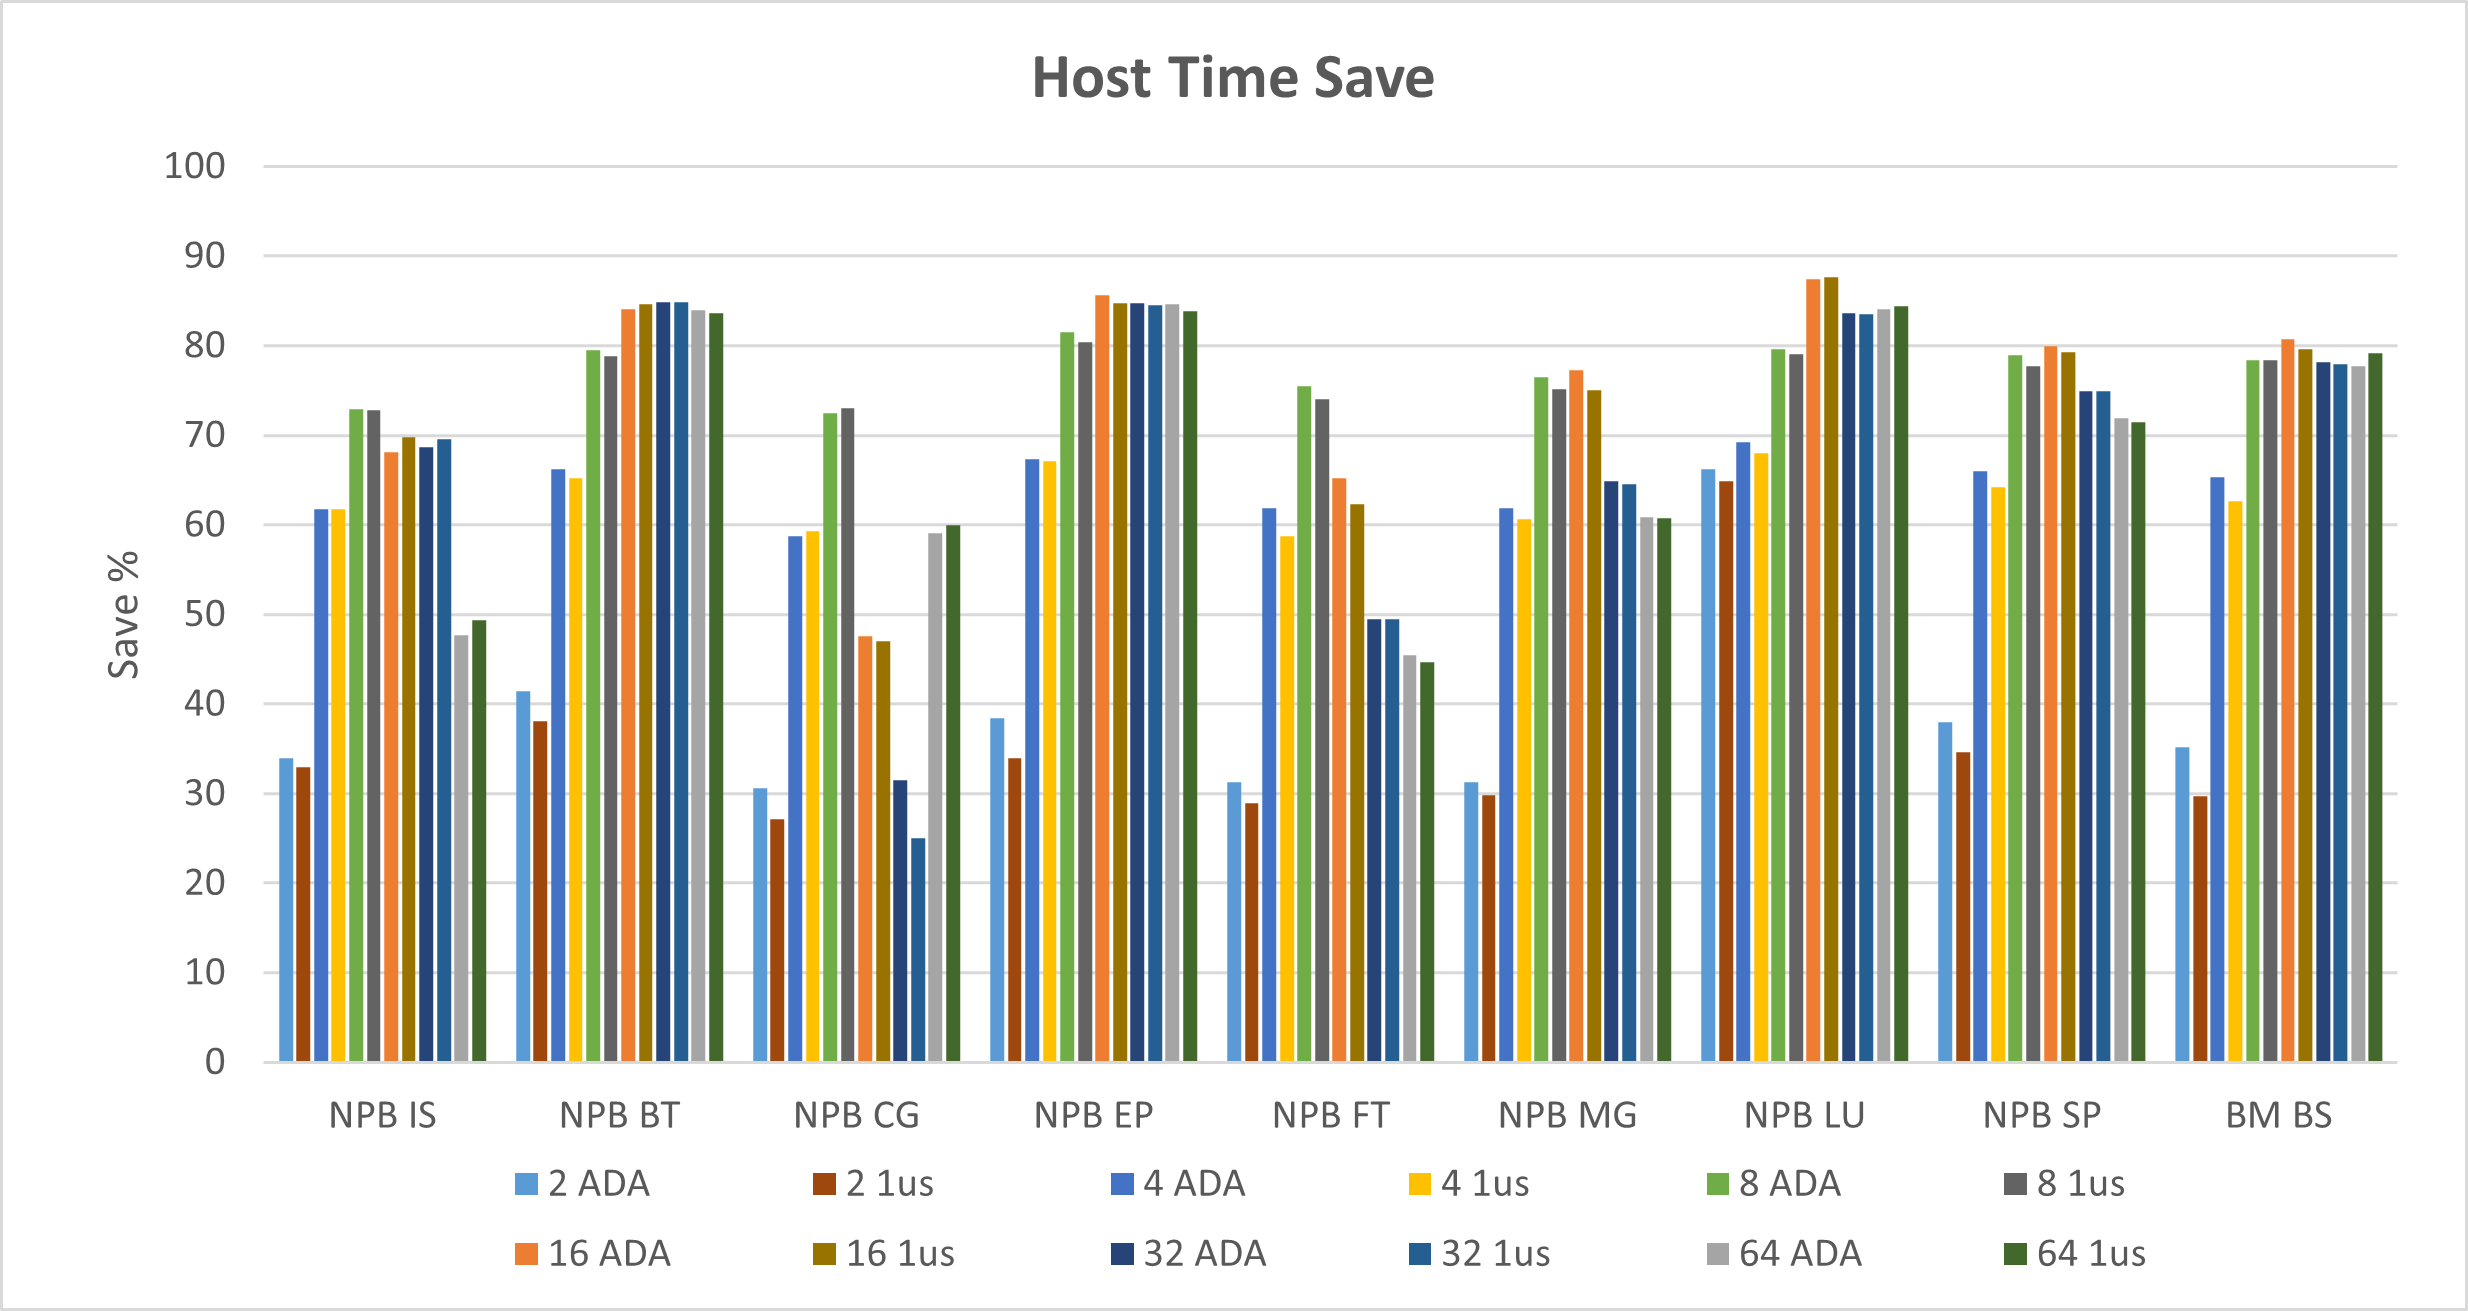
\includegraphics[width=0.75\textwidth]{Images/Host_ADA.png}
    \caption{ Host time save}
    \label{fig:Host_ADA}
\end{subfigure}
        
\caption{ADALINE algorithm results}
\label{fig:results_ADA}
\end{figure}

The horizontal subtitle illustrates the executed benchmark along with the number of cores and the corresponding algorithm used, hence 4 ADA means it were simulated four cores with the ADALINE algorithm. To assess the performance of ADALINE, the static version was also executed with a quantum set to 1 microsecond. In all cases, the comparison reference is the result obtained from sequential simulation. Additionally, the results for a single simulated core are not presented because in all conducted tests, the sequential simulation exhibited similar performance. Hence, this scenario is not relevant for evaluating the algorithms.

When it comes to performance, it's noticeable that the algorithm yielded better results in certain benchmarks such as baremetal, NPB EP, and SP. However, in other cases like NPB IS and CG, it did not show significant improvements. Shifting the focus to accuracy, the static version generally outperformed the dynamic approach. Nevertheless, the dynamic approach consistently maintained an accuracy of under 2\%, with the exception of NPB CG, where both approaches performed poorly. Lastly, when comparing the host time to performance, similar outcomes were observed, though certain benchmarks exhibited superior results to others.

This performance issue may be related with the previous quantum increment consideration. It is clear this value for some workloads is good, but for others may not be the most adequate. Therefore, having a dynamic value would solve this problem, resulting in more flexible algorithm. Moreover, special attention should be given to its design, as excessively large values can lead to an unfavorable trade-off.

%perguntar se nestes resultados intermedios coloco tb os de 32 e 64 ou no no "final" Incluir tambem os testes LU e SU? (Deixar em background e tentar mete-los)


\section{Increment Algorithm}

As shown, it was verified in some cases where the performance was equal or lower when compared with the static approach. Concerning the quantum increment, a fixed value was defined following the aforementioned philosophy however, a dynamic approach may bring better results, as different benchmarks require different needs. 

Therefore, the ADALINE algorithm was updated to integrate this new functionality. Observing the \autoref{fig_ADALINE_v1}, the calculation of the increment value (incValue) will be done before the if statement, so it can still be used in this quantum's calculation. The new flowchart is represented in the next figure.

\begin{figure}[H]
	\centering
 	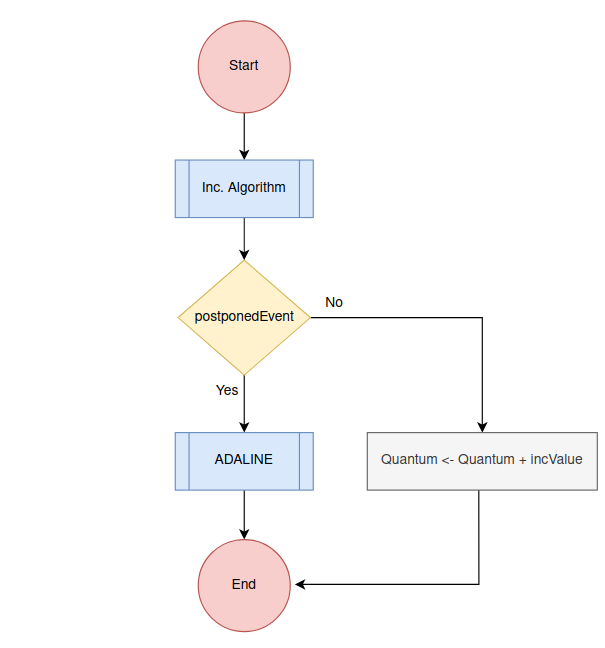
\includegraphics[width=0.5\linewidth]{Images/ADALINE_v2.png}
 	\caption{ADALINE with increment algorithm flowchart}
	 \label{fig_ADALINE_v2}
\end{figure}

The concept is to commence with a gradual increase in value initially. If there are no postponed events during this period, then the increment can be escalated. It can be seen as an exponential however, an approach like this would scale too fast, affecting the accuracy. A solution can be the definition of a threshold, where the increment value only increases if no accuracy issues have happened N times in a row. An example is illustrated in the \autoref{fig_incAlgorithm_graph}. 

\begin{figure}[h!]
	\centering
 	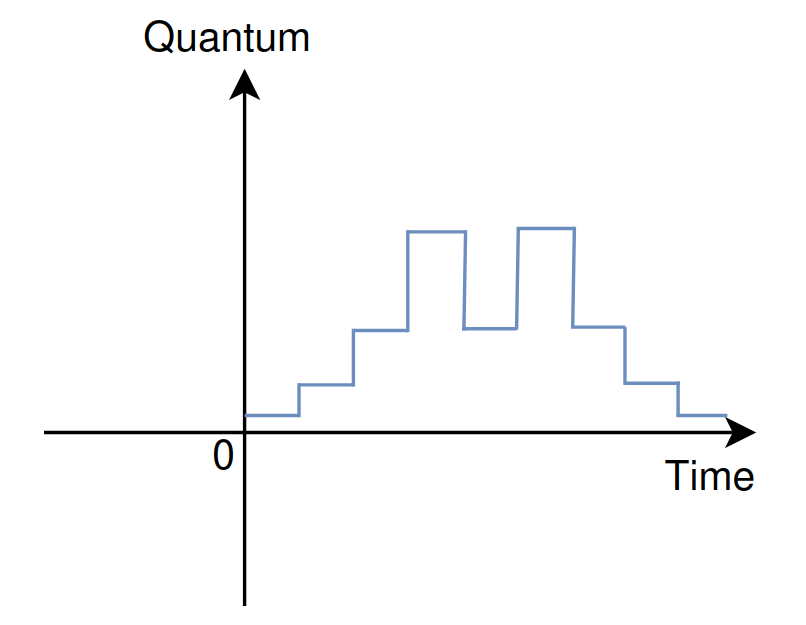
\includegraphics[width=0.5\linewidth]{Images/incAlgorithm_graph.png}
 	\caption{Example of evolution of the increment value with a threshold}
	 \label{fig_incAlgorithm_graph}
\end{figure}

The incValue starts in the smaller value possible, which is equal to the clock period, and grows until it reaches a maximum, that is 100 microseconds. It was defined regarding the results on \cite{pargem5} and \cite{BeyondQuantumTDSim}, where the benefits of a quantum of this magnitude are few. The addition method respects the subsequent equation.

\begin{equation}
    \label{eq_incValue}
    \centering
        \Large
        incValue = 2 * incValue
        \normalsize
\end{equation}
\vspace{0.3cm}

Oppositely, the decrement is done by dividing by two the actual incValue, until it reaches the minimum. The threshold value depends on how many cores are used by the simulation since the inaccuracy grows with the increasing number of cores. The more cores are being used, the greater the threshold. Moreover, the increment value only changes (increases or decreases) if it fulfills the condition for N consecutive times. The later image shows the algorithm's flowchart. 

\begin{figure}[H]
	\centering
 	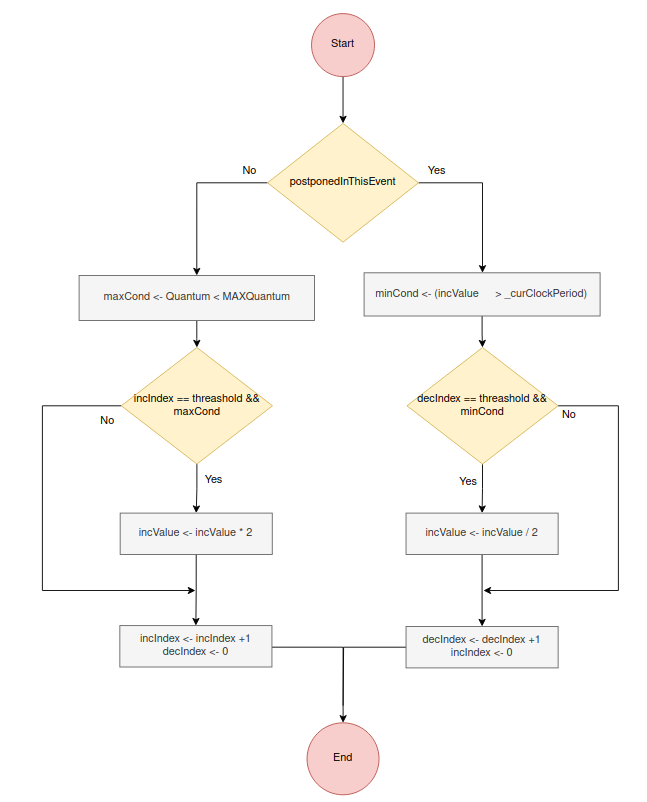
\includegraphics[width=0.7\linewidth]{Images/incAlgorithm_flowchart.png}
 	\caption{Increment algorithm flowchart}
	 \label{fig_incAlgorithm_flowchart}
\end{figure}

\subsection{Results}

The previous benchmarks executed the new approach with different number of cores. The results obtain are depicted in the \autoref{fig:results_ADAINC}. 

\begin{figure}[H]
\centering
\begin{subfigure}{\textwidth}
    \centering
    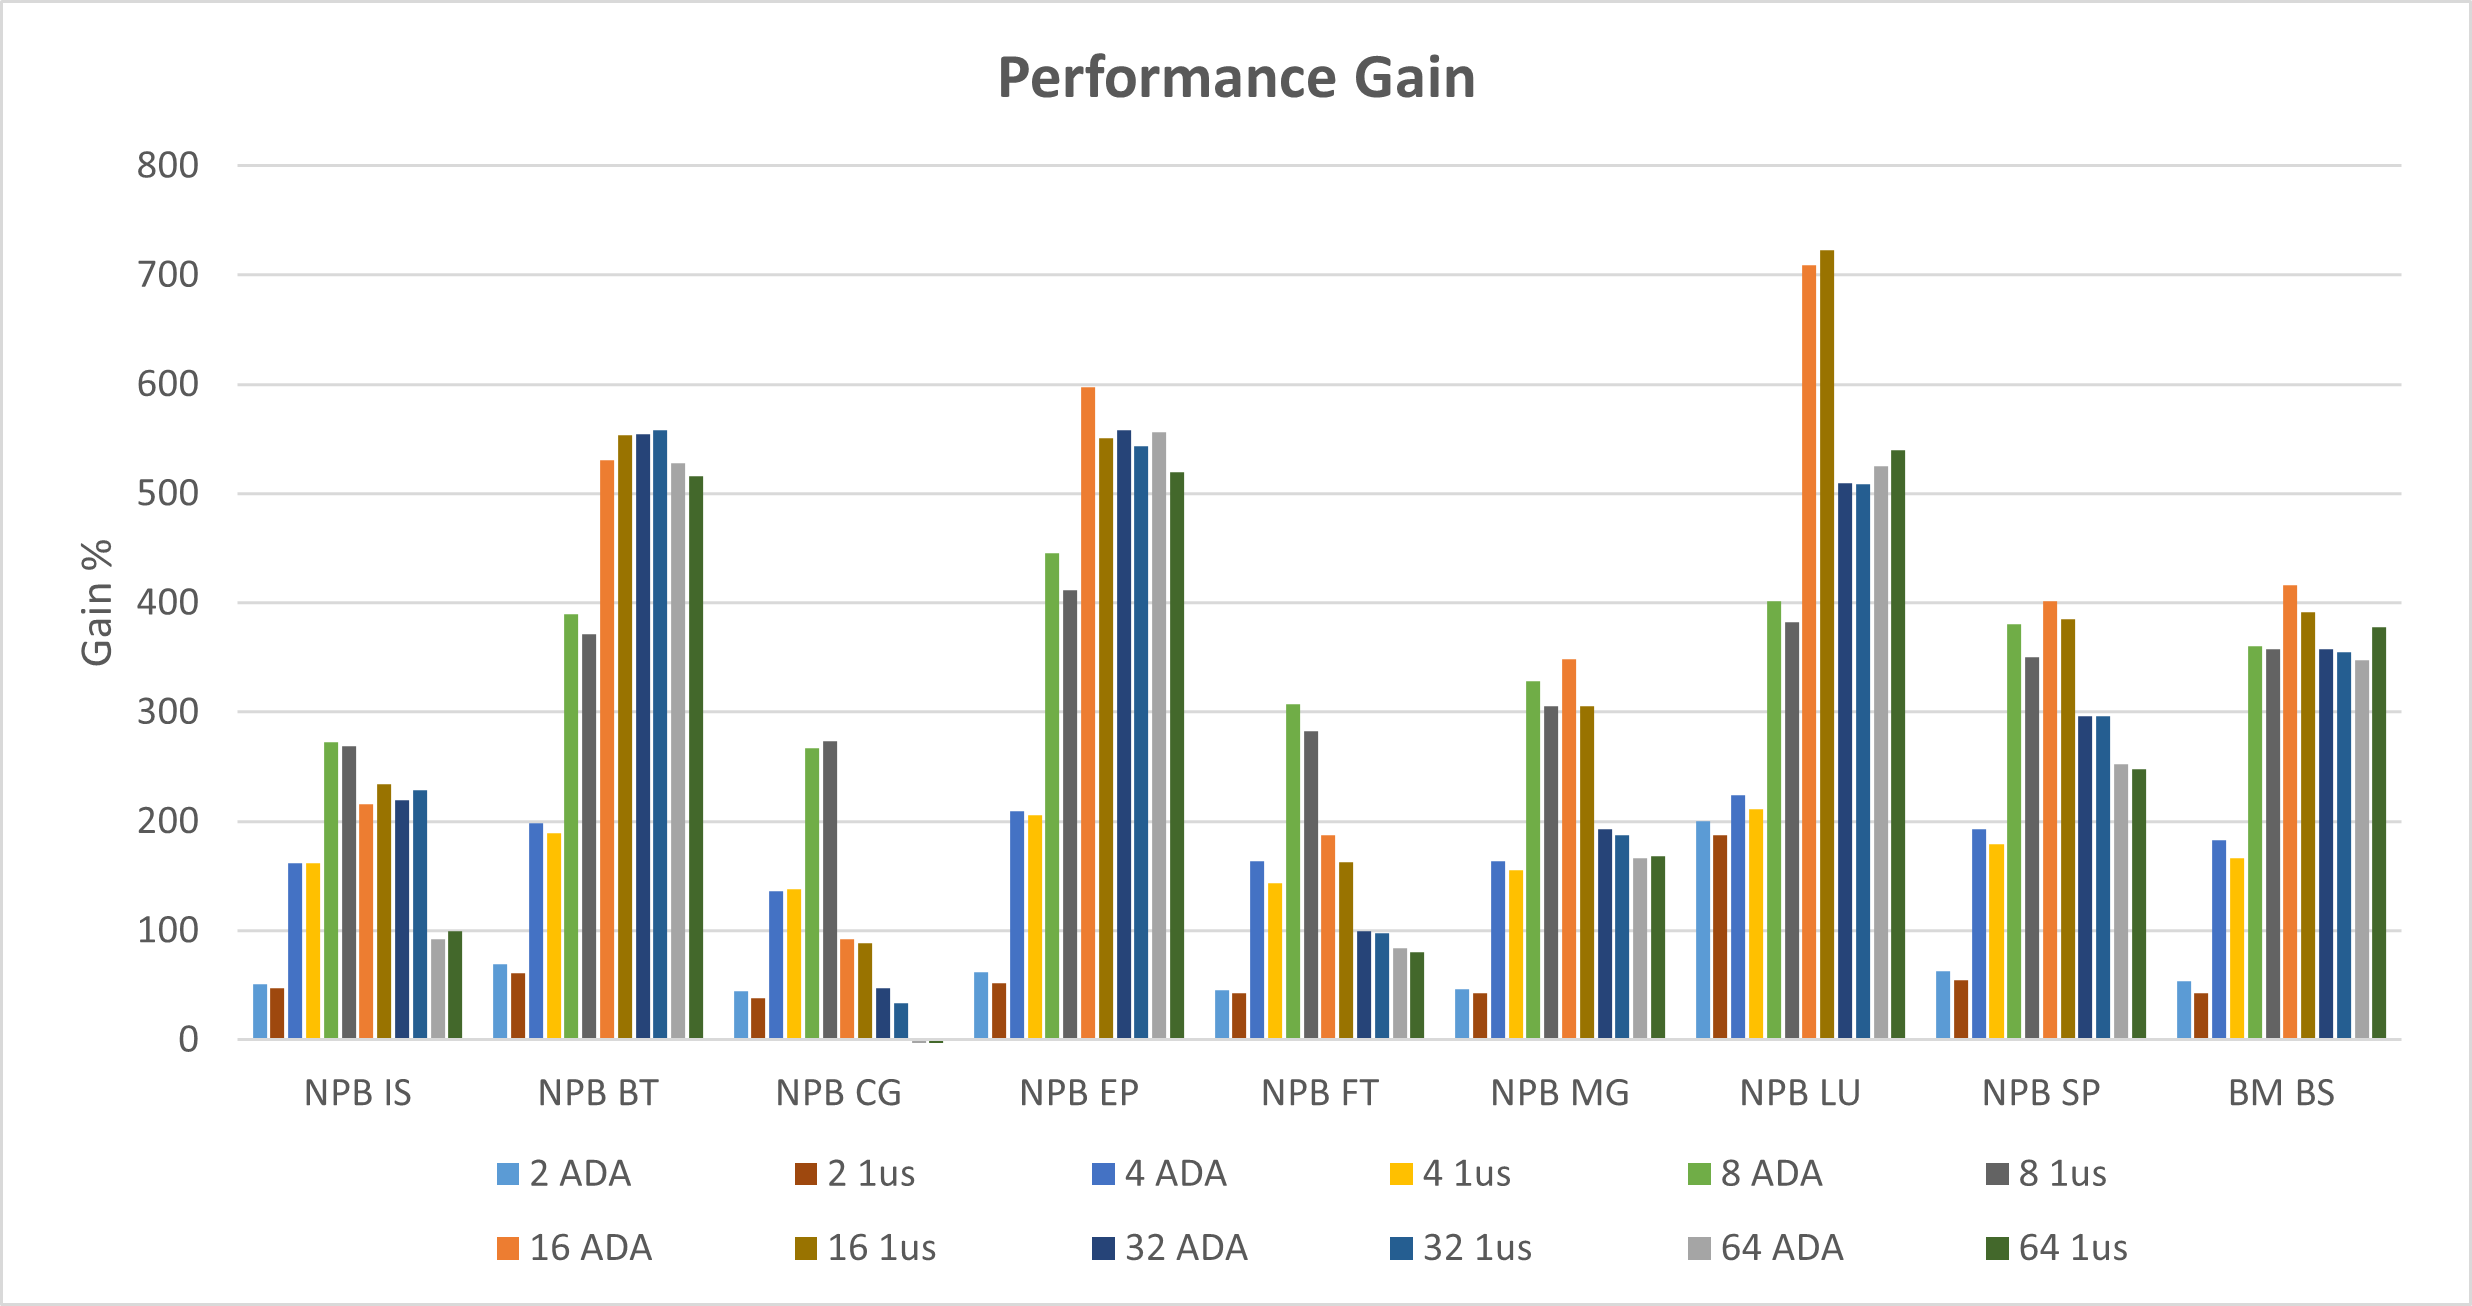
\includegraphics[width=0.75\textwidth]{Images/Performance_ADA.png}
    \caption{ Performance gain}
    \label{fig:Performance_ADAINC}
\end{subfigure}
\begin{subfigure}{\textwidth}
    \centering
    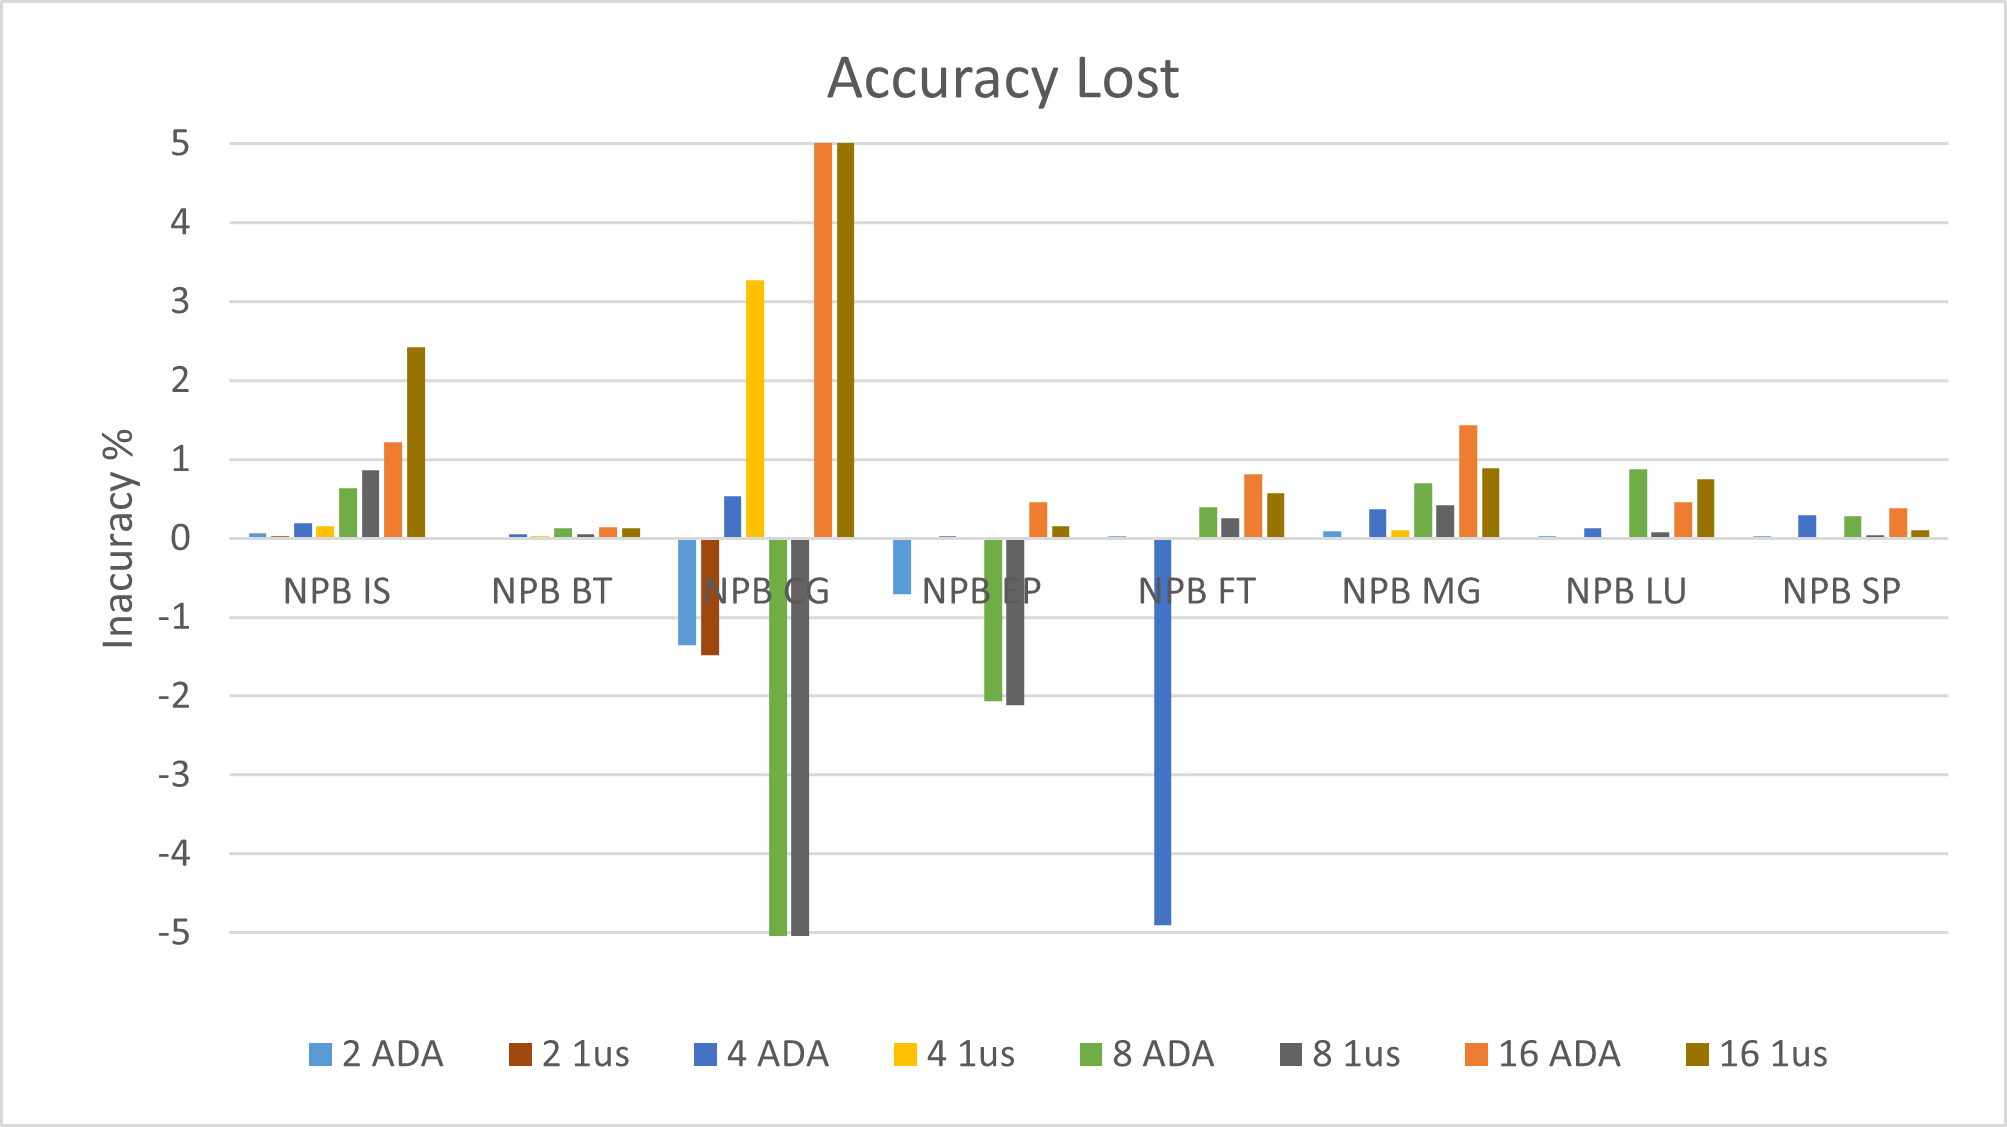
\includegraphics[width=0.75\textwidth]{Images/Accuracy_ADA.png}
    \caption{ Accuracy lost}
    \label{fig:Accuracy_ADAINC}
\end{subfigure}
\begin{subfigure}{\textwidth}
    \centering
    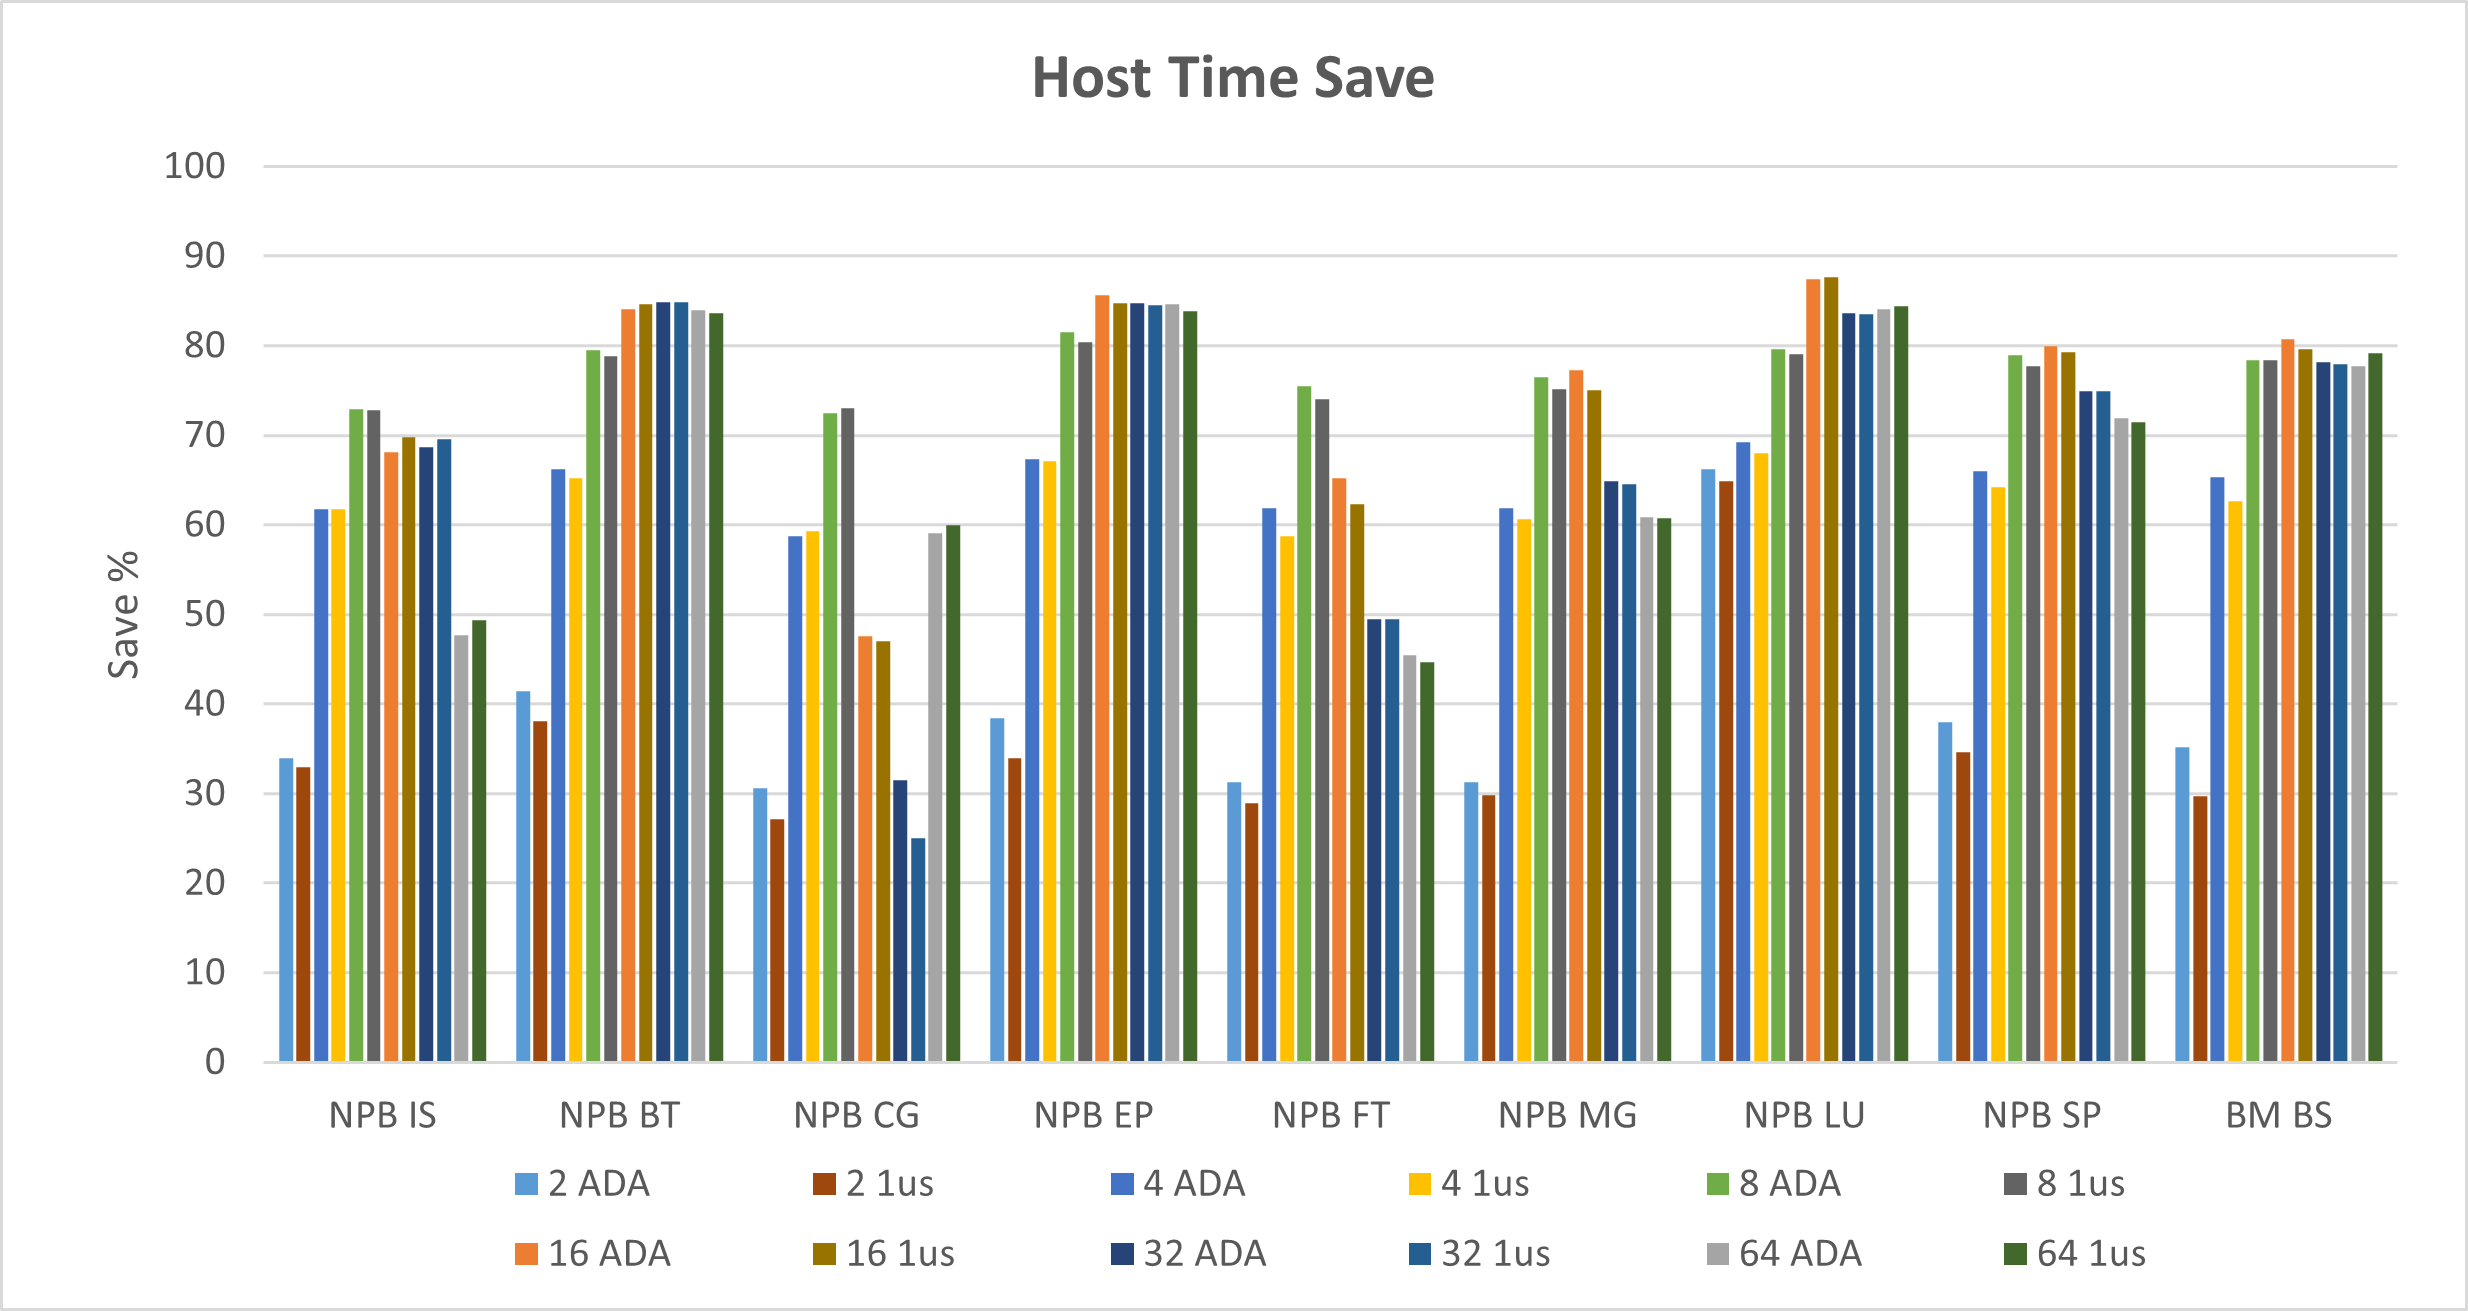
\includegraphics[width=0.75\textwidth]{Images/Host_ADA.png}
    \caption{ Host time save}
    \label{fig:Host_ADAINC}
\end{subfigure}
        
\caption{Dynamic increment results}
\label{fig:results_ADAINC}
\end{figure}

%Fazer a conta de quanto aumento a performance, accuracy e host
\textbf{The ADA refers to the first results, while A-I is related to the new configuration. As expected, the dynamic approach in the increment value resulted in better performance. On average, the performance increment was about ....... Additionally, as a consequence of that, the host time was lower, reducing it by ...... }

Unfortunately, the same did not occur in terms of accuracy. In all cases, except for the NPB.LU benchmark with sixteen simulated cores, there was a reduction. In some cases, such as the NPB.FT and NPB.EP with sixteen simulated cores, experienced a significant drop, with accuracy falling below 95\%. A possible explanation for this could be the nature of the algorithm itself. The adaptive filter may not be designed to handle drastic interventions. As shown in \autoref{fig:AF2}, the control action appears to be smooth, even though there are moments, for example, in inter-process communications when it should be more aggressive to prevent postponed events in cross-scheduling. The problem was not evident at the beginning, however, with the dynamic increment, it becomes more notable. 

One of the requirements for this dissertation is to maintain a maximum inaccuracy of 5\%, thus the current approach does not meet this criterion. It is crucial to explore alternative methods and optimizations to ensure that the desired level of accuracy is achieved.

\section{PC Algorithm}

As mentioned before, one problem of the previous algorithm is the incapability to reduce the quantum significantly in a short period. A potential solution for this issue could involve predicting when this situation is likely to occur. In other words, an attempt can be made to assess when a postponed event will take place. If it becomes possible to forecast when such an event will be postponed, adjustments can be made to the quantum before it happens. This preemptive action can help prevent significant inaccuracies from occurring. 

Before the simulation initiates, the commands destined for execution are loaded into memory and remain unaltered throughout the simulation. These, when executed, can lead to a postponed event. An example of that is the Wait for Event (WFE) instruction, where the \gls{cpu} enters in low-power standby state. Furthermore, in general, loops are the backbone of benchmarks, whether due to multiple iterations or the benchmark's inherent characteristics, such as testing the transfer of memory blocks between different locations. As a result, the same instruction address can be encountered more than one time. 

By evaluating the \gls{pc}, it is possible to understand if the processing of one instruction can result in a postponed event (PPaddr), and so avoid its execution with a large quantum. With this idea in mind, the \gls{pc} algorithm, as the name suggests, will analyse the \gls{pc} during the simulation, in order to perform the prediction of when these instructions will be executed. \autoref{fig_PCAlgorithm} exemplifies an example how the algorithm works.

\begin{figure}[h!]
	\centering
 	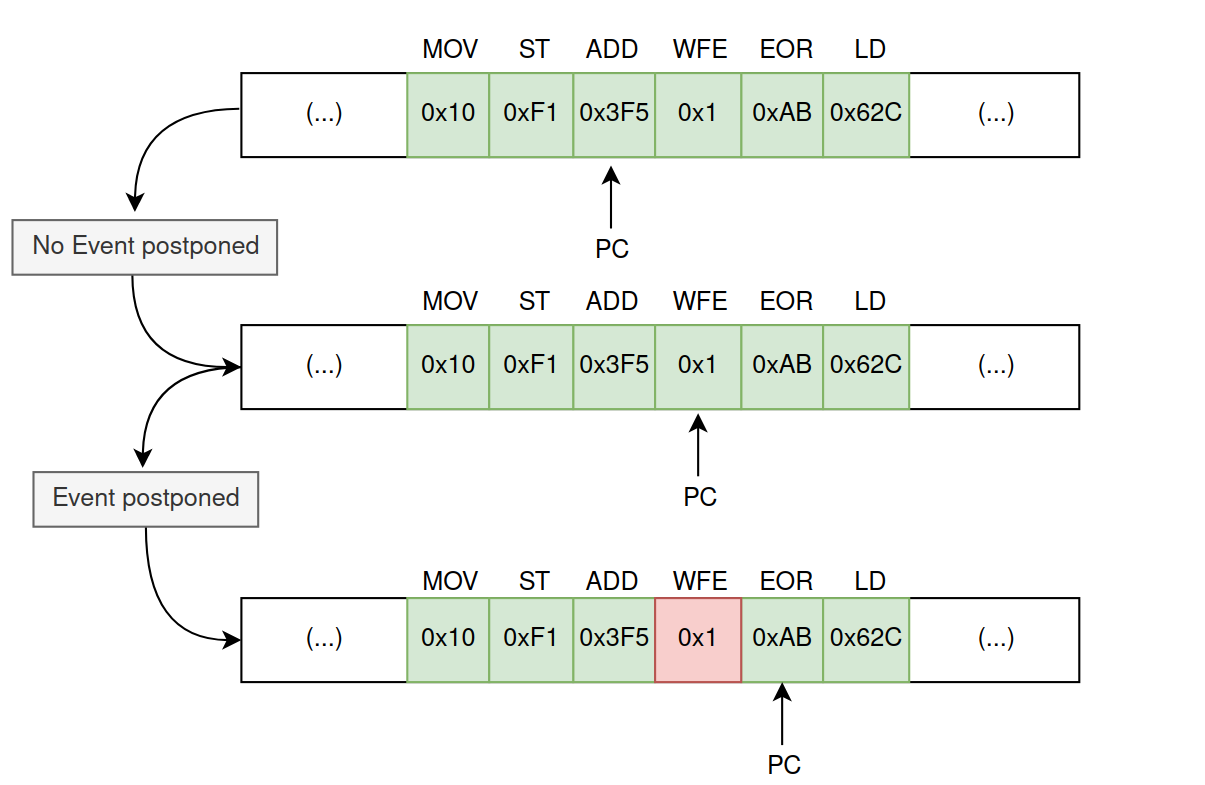
\includegraphics[width=0.7\linewidth]{Images/PCAlgorithm.png}
 	\caption{PC Algorithm}
	 \label{fig_PCAlgorithm}
\end{figure}

In the beginning, every instruction is considered risk-free, but as the simulation proceeds, it can be changed. When it happens, the processed instruction becomes a spotted address, marked in red in the figure, until the end of the simulation. All these addresses will be taken into account in the new quantum calculation, thus these should be acknowledged as genuine "postponed event generators".


%Explicar o porque de so se considerar um spotted addr quando ocorrer 4 vezes



 
\subsection{Forecast}

Workloads are not straightforward in a way that the \gls{pc} do not follow a linear path. Instructions like "jump" (JMP) or interruptions have the potential to redirect the execution flow to different memory locations. Understanding exactly what type of instructions the simulator will execute and tracking them is computationally heavy, meaning performance costs. Since the algorithm should be lightweight, it is considered that the \gls{pc} is linear, that is, the next \gls{pc} will be the actual plus the instruction width. 

First of all, is used an analytic method to find where the program counter will be in the future. As a result of the previous consideration, the \autoref{eq_PCForecast1} was developed.

\begin{equation}
    FPC = PC + \left( \frac{Quantum * InstWidth}{CyclePeriod} \right)
    \label{eq_PCForecast1}
\end{equation}

\begin{equation}
    Quantum = \frac{  \left( FPC - PC \right) * CyclePeriod)}{InstWidth} 
    \label{eq_PCForecast2}
\end{equation}

Thereafter, one of two scenarios can unfold, as depicted in the next pictures. First, nothing may transpire if no addresses are identified between the \gls{pc} and FPC (Forecasted Program Counter). Alternatively, if the FPC corrects its value to the nearest identified address, a quantum recalibration is necessary, achieved using \autoref{eq_PCForecast2}. Hence, the synchronization will occur right after the execution of the spotted address, avoiding inaccuracy as the cross-schedule event is inserted in the target event queue at the expected time.

\begin{figure} [H]
\centering
\begin{subfigure}{\textwidth}
    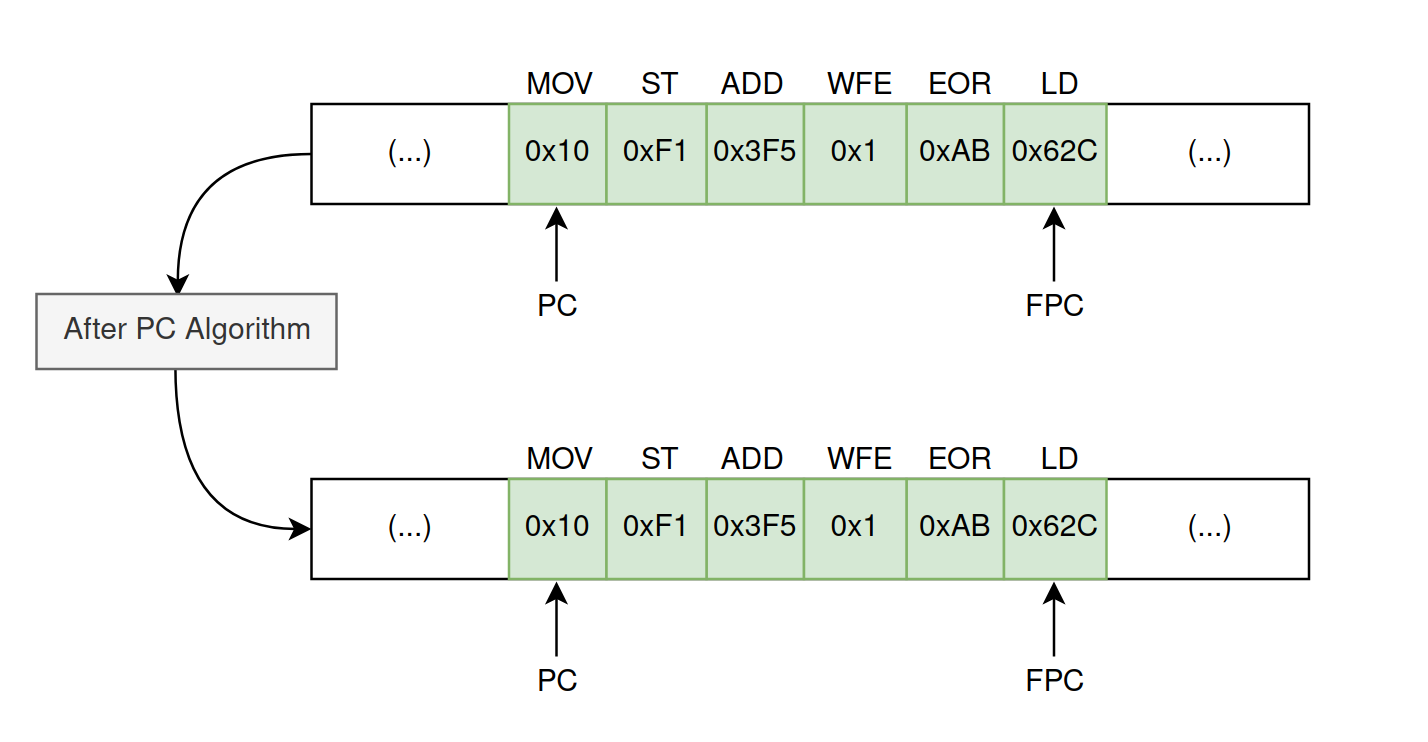
\includegraphics[width=0.8\textwidth]{Images/PCAlgrithm_noCut.png}
    \caption{ Scenario 1 }
    \label{fig:PCAlgrithm_noCut}
\end{subfigure}
\begin{subfigure}{\textwidth}
    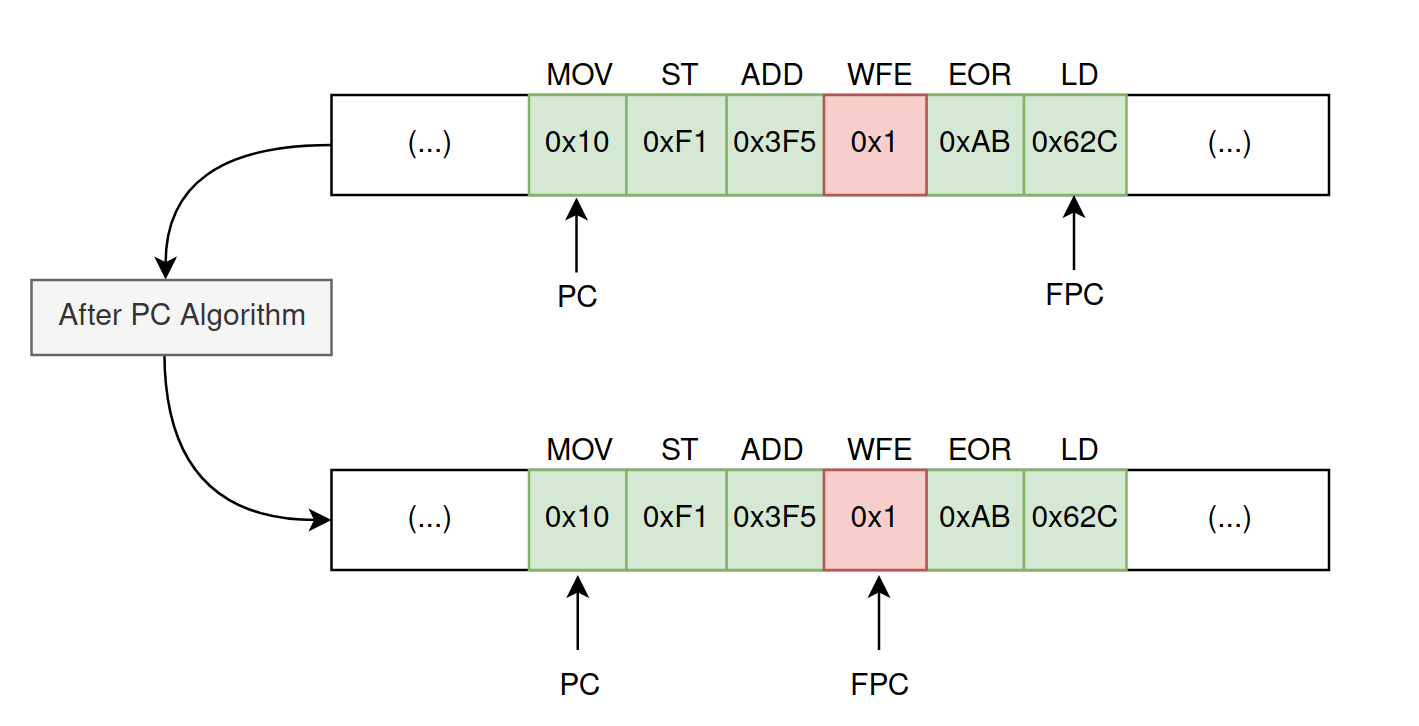
\includegraphics[width=0.8\textwidth]{Images/PCAlgrithm_Cut.png}
    \caption{ Scenario 2 }
    \label{fig:PCAlgrithm_Cut}
\end{subfigure}
        
\caption{Possible scenarios after the forecast}
\label{fig:PCAlgorithm_differentScenarios}
\end{figure}

\subsection{Increment Algorithm Update}

With the development of this new algorithm, there is a new way to verify whether the quantum is reduced, meaning the old one was greater than the desirable. By this reason, the increment algorithm will also verify this situation, counting as "inaccuracy problem", contributing for the reduction of the increment value.

To determine whether the previous scenario occurred, the quantum value before the PC algorithm's action is stored and compared to the current. If the stored value is equal to or higher than the current quantum, no action is taken. However, if the stored value is lower, it indicates that the quantum was reduced, triggering the flag. 


\subsection{Results}

The results of the bare-metal bubble-sort and \glspl{npb} benchmarks execution are presented in the \autoref{fig:results_ADAINCPC}. As previously, A-I refers to the ADALINE with the increment algorithm results, and A-I-P points to the results with the \gls{pc} algorithm intervention. 

\begin{figure}[H]
\centering
\begin{subfigure}{\textwidth}
    \centering
    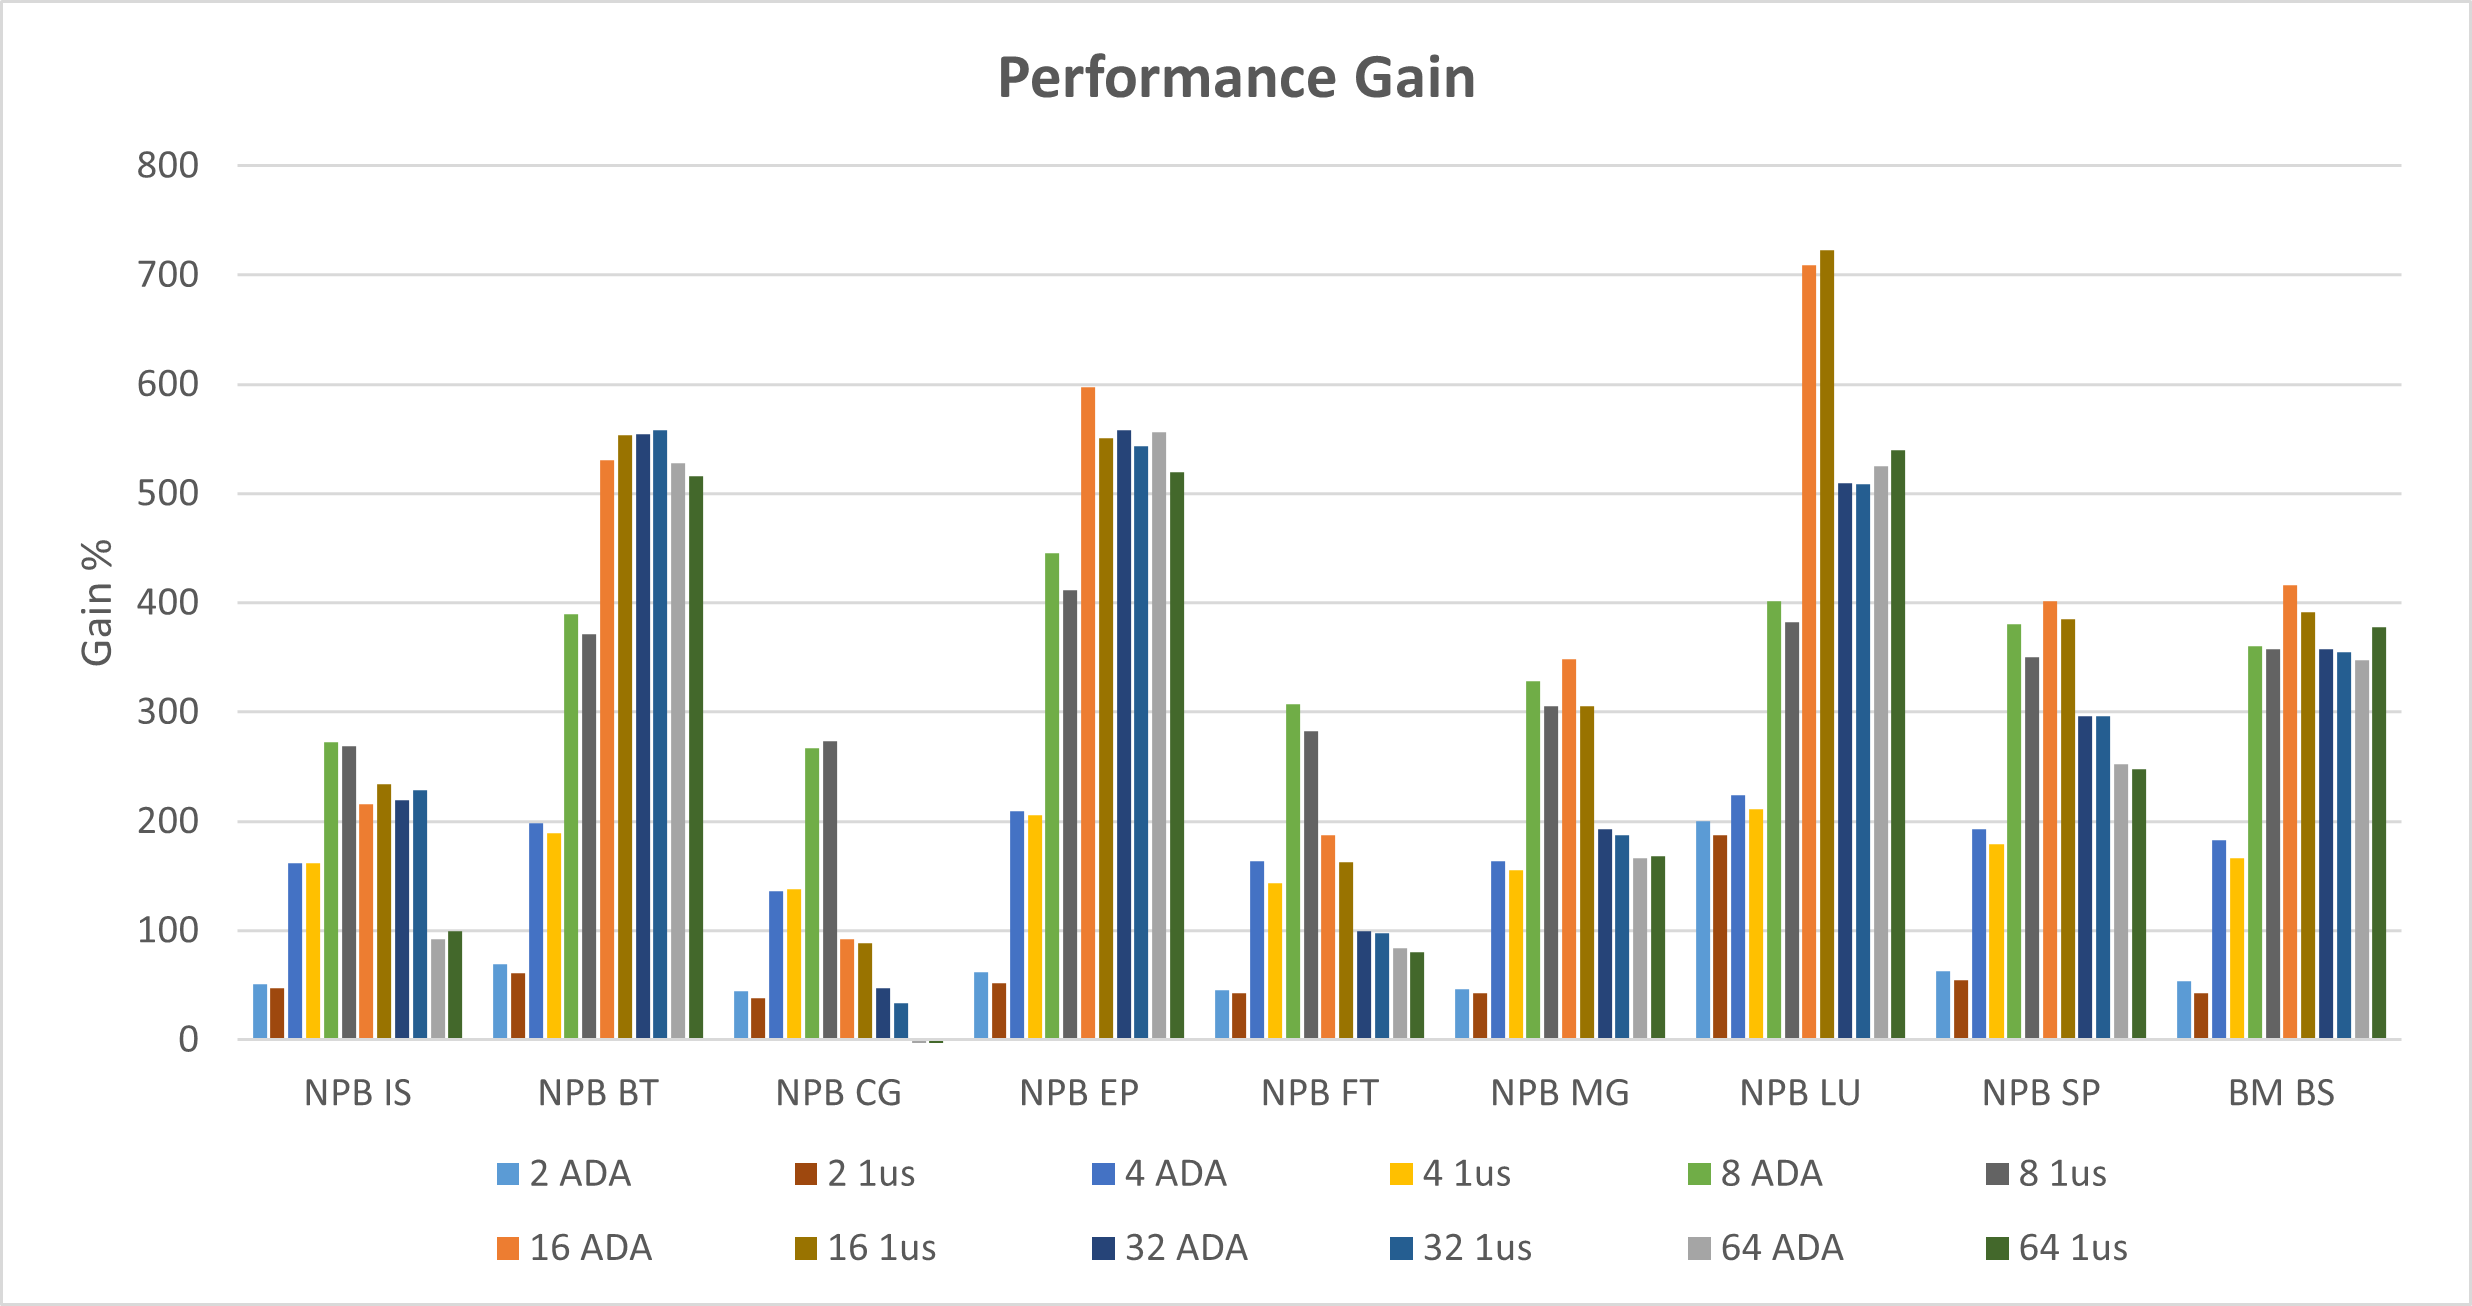
\includegraphics[width=0.75\textwidth]{Images/Performance_ADA.png}
    \caption{ Performance gain}
    \label{fig:Performance_ADAINCPC}
\end{subfigure}
\begin{subfigure}{\textwidth}
    \centering
    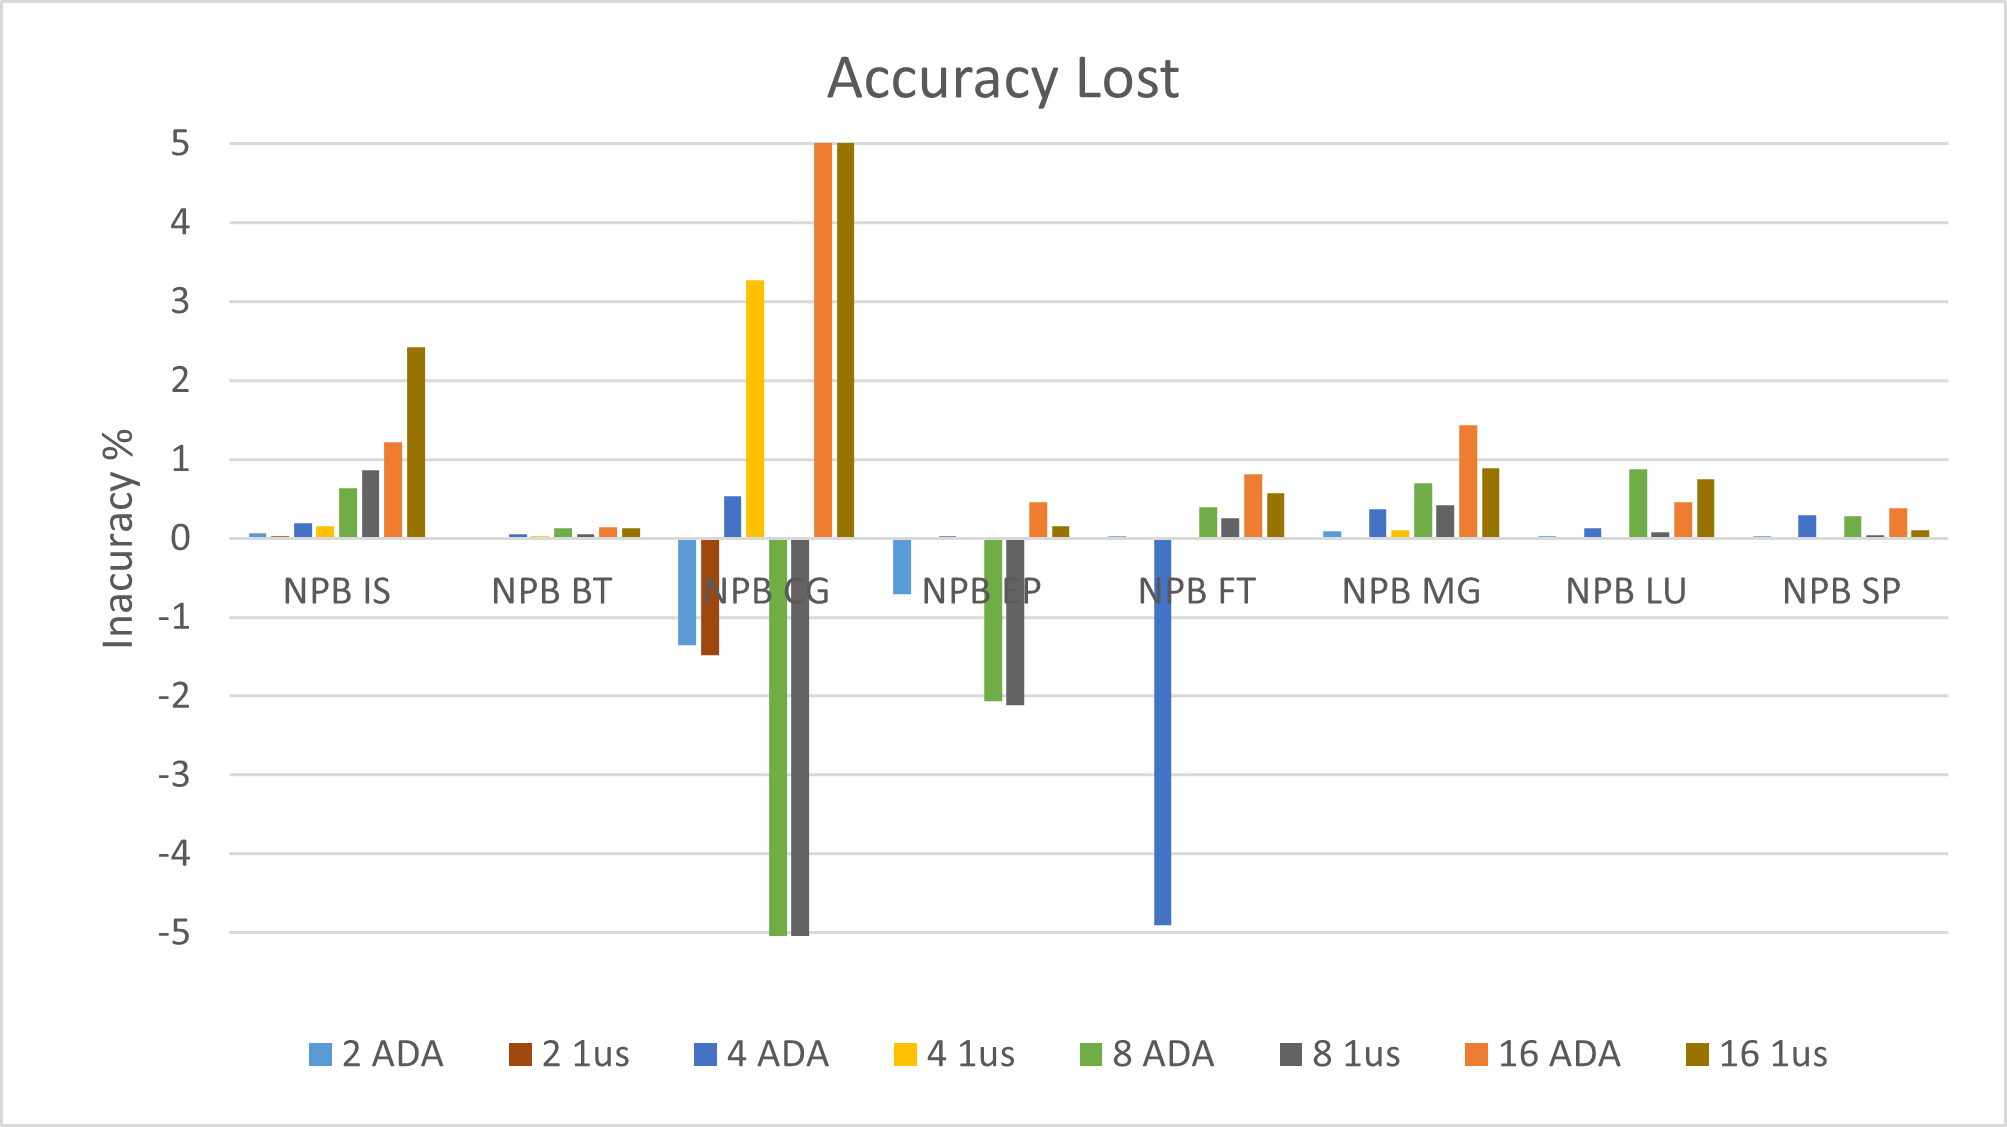
\includegraphics[width=0.75\textwidth]{Images/Accuracy_ADA.png}
    \caption{ Accuracy lost}
    \label{fig:Accuracy_ADAINCPC}
\end{subfigure}
\begin{subfigure}{\textwidth}
    \centering
    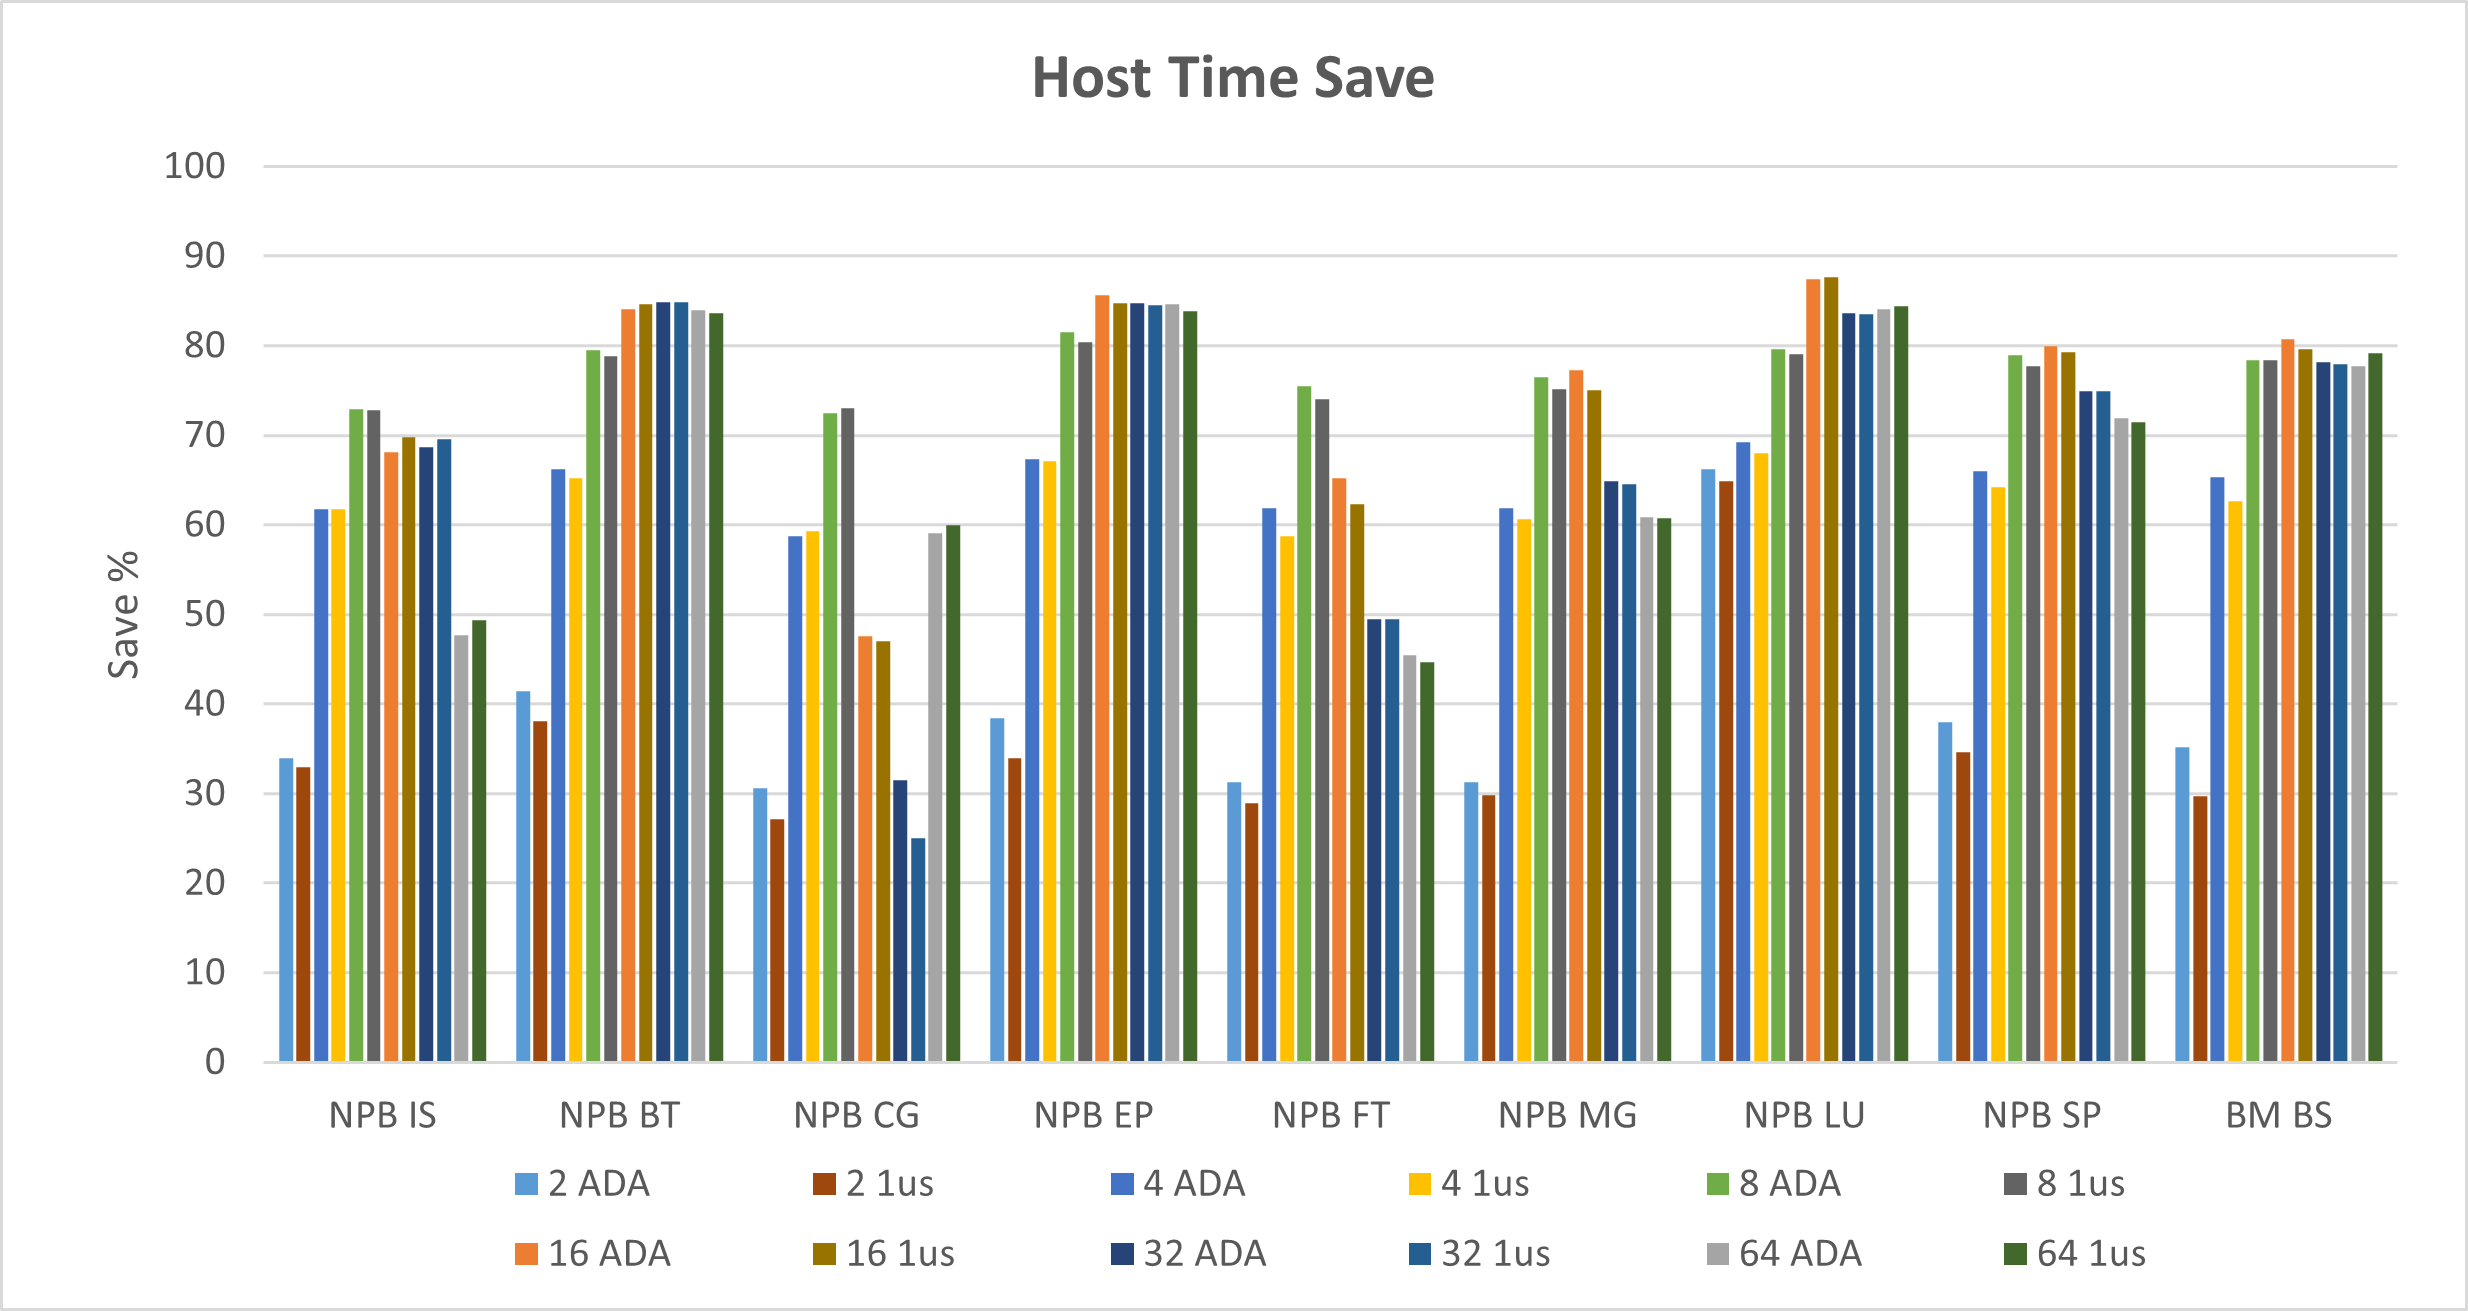
\includegraphics[width=0.75\textwidth]{Images/Host_ADA.png}
    \caption{ Host time save}
    \label{fig:Host_ADAINCPC}
\end{subfigure}
        
\caption{\gls{pc} algorithm results}
\label{fig:results_ADAINCPC}
\end{figure}

Starting with the performance gain, it did not have a significant drop, only about  ......... \%. In practice, in most workloads this reflected in an increment of the host time of ...... seconds approximately. Nevertheless, there are a few cases in the algorithm's action conducted into better performance, in particular the NPB.BT over eight simulated cores. 

The most distinguished side is the accuracy, where the \gls{pc} algorithm inclusion allowed an inaccuracy reduction of ....... \%. The previously mentioned cases that passed the 5\%, are now within the limit. Moreover, analyzing the worst case of accuracy loss, a reduction can be seen in most scenarios.  

\begin{figure}[H]
	\centering
 	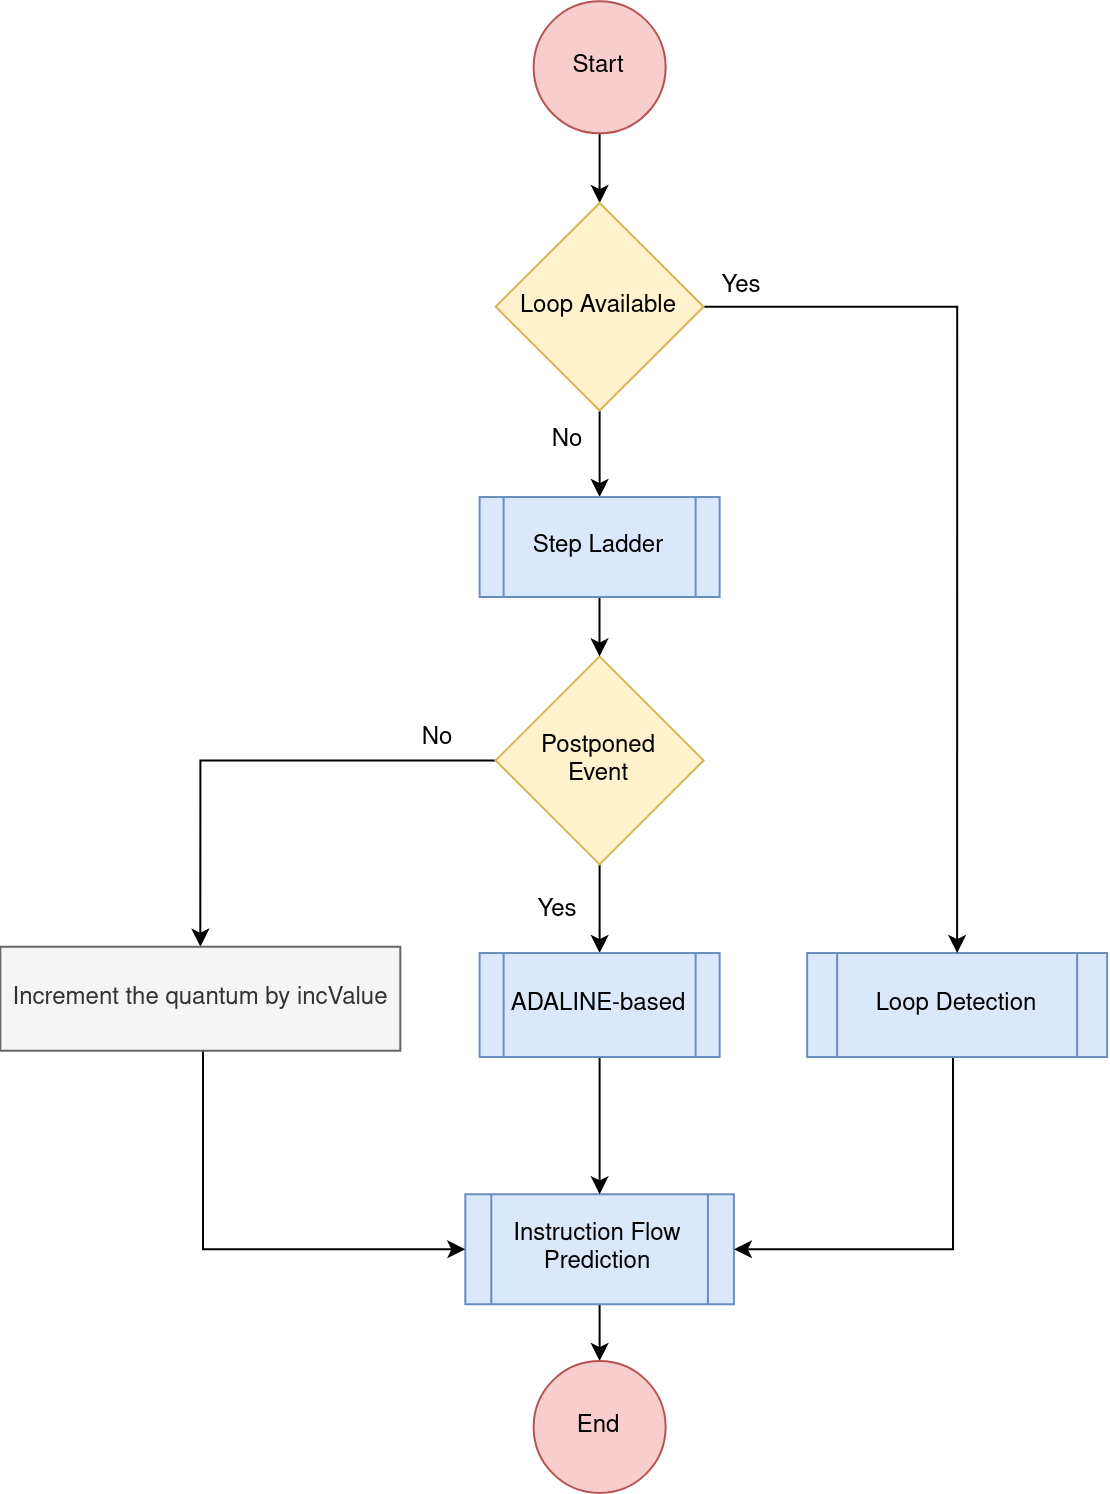
\includegraphics[width=0.5\linewidth]{Images/ADA_and_REP.png}
 	\caption{Worst case of accuracy lost comparison}
	 \label{fig_WorstCase_PC}
\end{figure}



\section{Repetition Algorithm}

As mention earlier in this chapter, loops are strongly present in benchmarks. Thinking in this perspective, if a record of every executed instruction is made, a loop can be identified in real-time. Combining this with the previous algorithms, the quantum could be adapt in a way to have the higher value possible. Furthermore, the accuracy would be nearly perfect since all cross-schedule events would be known, allowing for precise adaptation.


\begin{figure}[h!]
	\centering
 	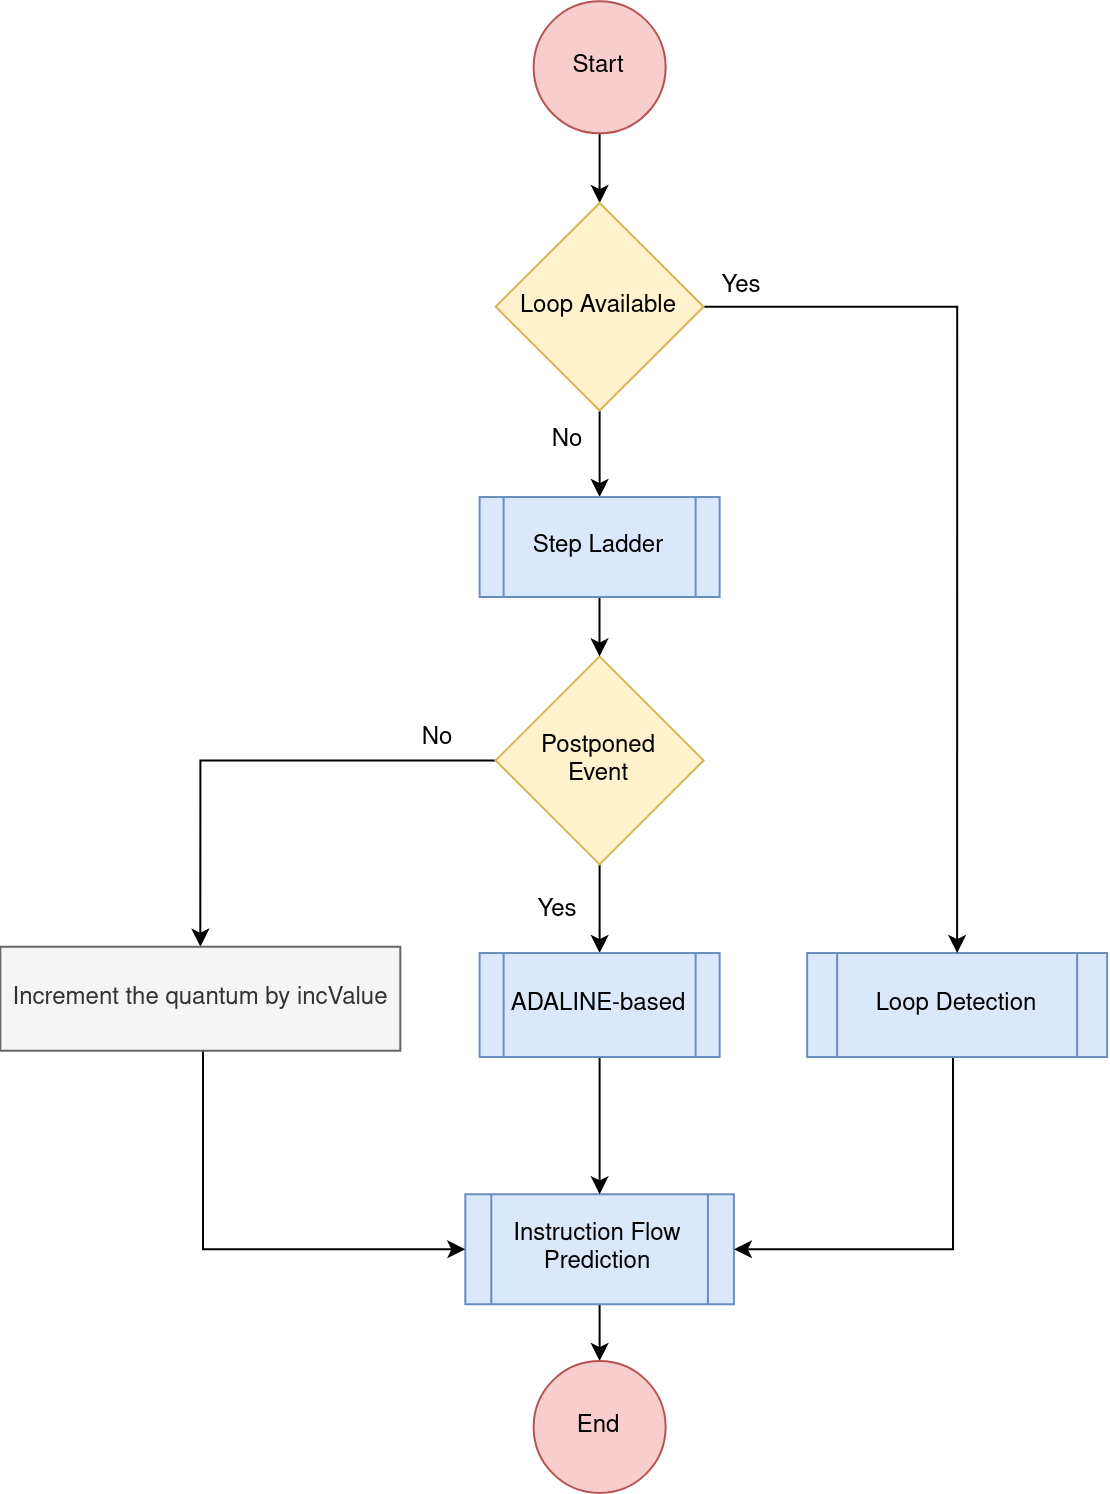
\includegraphics[width=0.5\linewidth]{Images/ADA_and_REP.png}
 	\caption{Quantum definition with repetitions algorithm}
	 \label{fig_ADA_and_REP}
\end{figure}


When the simulation starts, there are no information about loops or PPaddrs. To have this it would be needed to execute the simulation once and then obtain the results, what does not match with the requirements. One solution is to conduct the simulation in a regular manner while simultaneously recording the executed instructions. When a loop is detected, the algorithm begins utilizing the loop to calculate the quantum until the \gls{pc} no longer follows the loop's path. At that point, the loop is reset, and the process starts anew.

\subsection{Hare-Tortoise Algorithm}

The detection method must be light, otherwise the simulation performance is set in danger. One algorithm with this characteristic is the Floyd's Tortoise and Hare technique. It consists in two pointers, one twice faster than the other. If the two match at some point, means that there is a loop, as shown in the figure bellow.

\begin{figure}[H]
	\centering
 	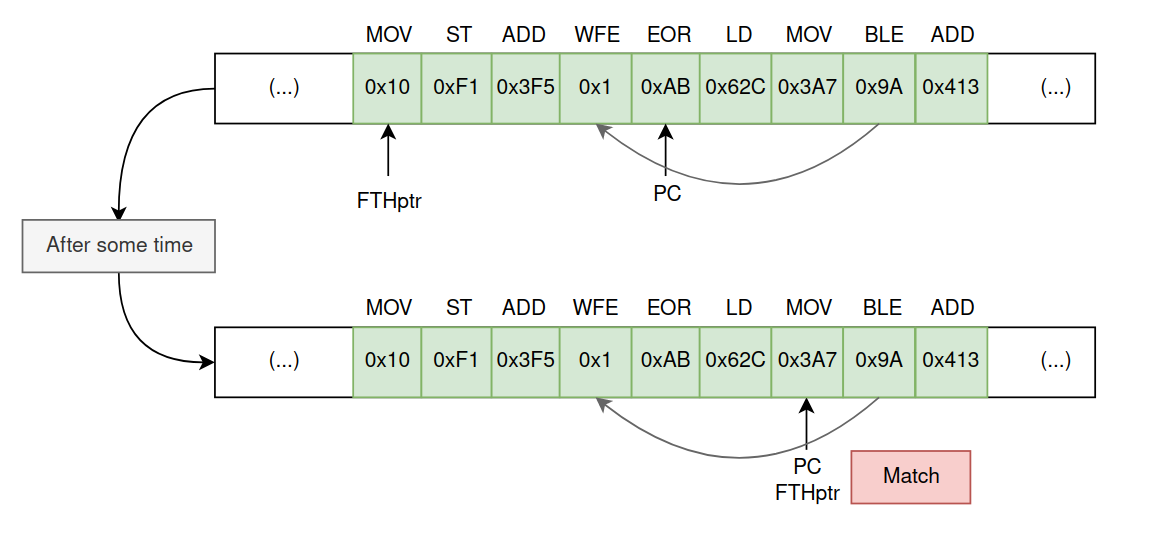
\includegraphics[width=0.8\linewidth]{Images/FTH_algorithm.png}
 	\caption{Hare-Tortoise Algorithm}
	 \label{fig_FTH_algorithm}
\end{figure}

In this case, the faster pointer is the \gls{pc}, and the slower one is the FTHptr. A match occurs when both are pointing to the same memory at the same time. To delve further into the process, loop delineation can be achieved through two methods. Firstly, an analysis can be conducted on the preceding instruction to precisely define the loop boundaries. Alternatively, after the initial match, the FTHptr remains in the same position while the \gls{pc} continues execution. When they match once more, the loop becomes well-defined. In terms of performance, it is trivial the second approach is more underweight, reason why it was chosen. After the detection, it is necessary to keep track of the \gls{pc}, as referred earlier. It is done by comparing the actual \gls{pc} with the expected one. Whether matches, nothing happens. In the opposite way, the loop is discarded and the hole process of detection starts again. The flowchart present in the \autoref{fig_Repetition_flowchart} describes the detection flow. 

\begin{figure}[h!]
	\centering
 	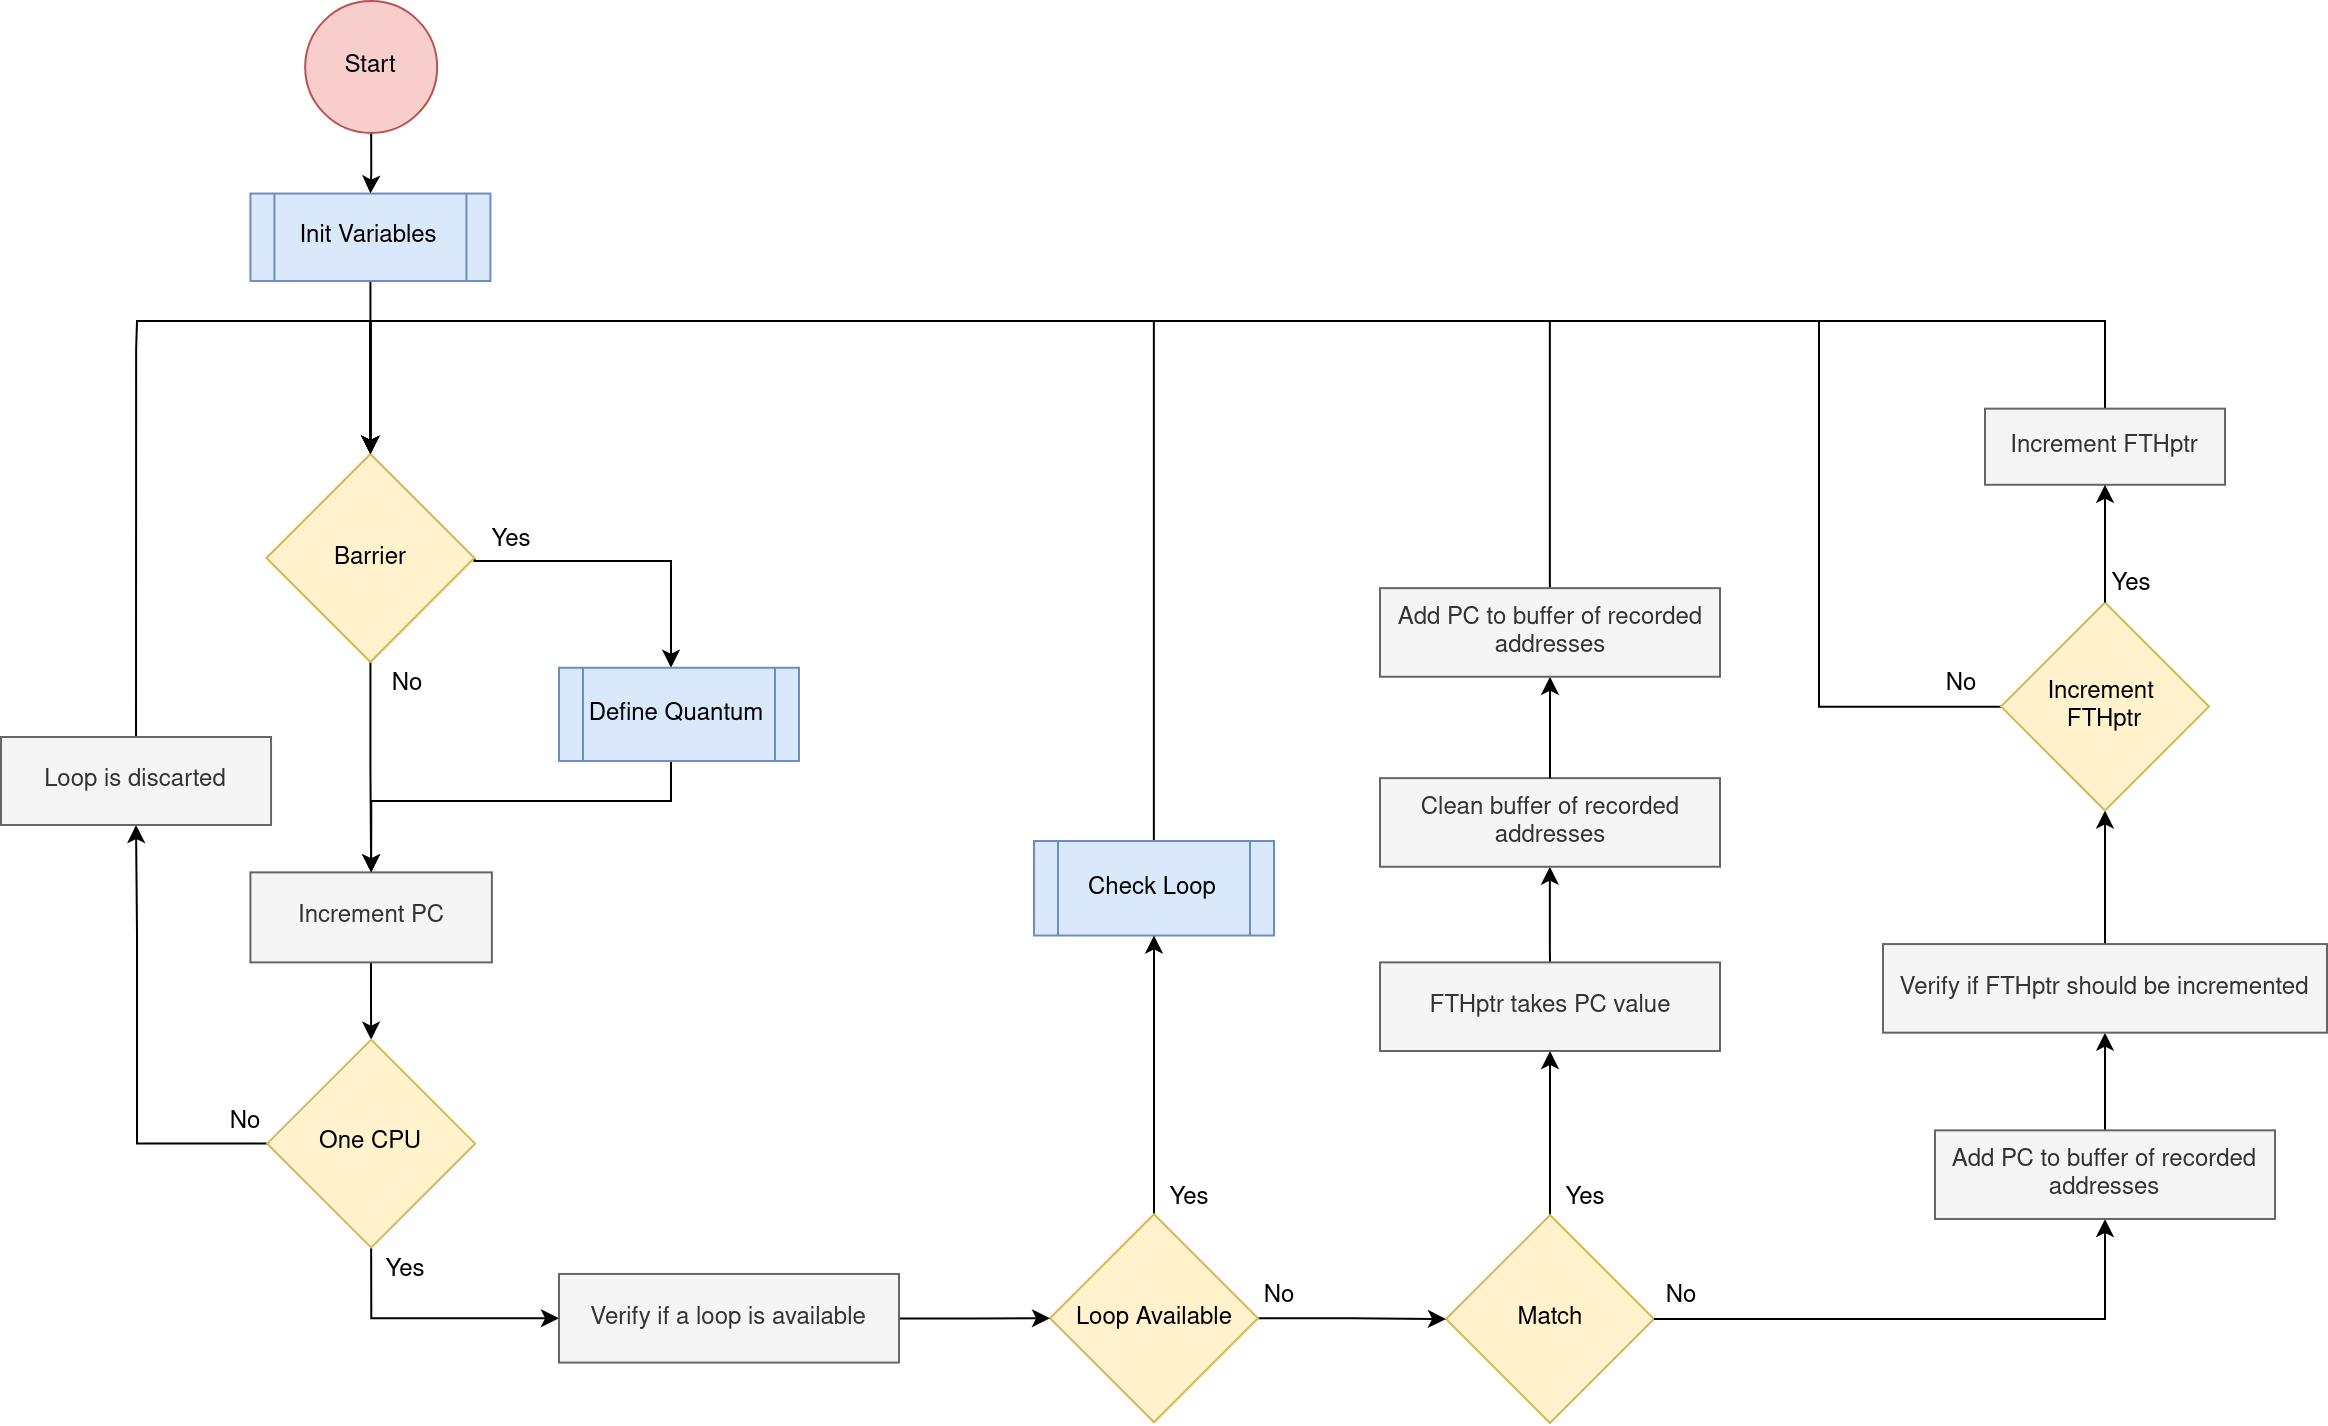
\includegraphics[width=1\linewidth]{Images/Repetition_flowchart.png}
 	\caption{Loop detection flowchart}
	 \label{fig_Repetition_flowchart}
\end{figure}


Although this technique is simple and very effective, it has some inherent problems. The first issue pertains to the inability to detect nested loops. Another challenge is the incapability to identify subsequent loops following the one that has been detected. The most crucial problem is the difficulty in detecting conditions within loops. All of these can be solved with the \gls{pc} track nevertheless, these solution may cut the benefits of the algorithm, since these problems can be recurrent in the benchmark. 

Another problem is the multi-thread environment. When more than one \gls{cpu} is active, the \gls{pc} executes more than one event queue, meaning an unpredictable pointer. In this situation is mostly impossible to identify any loop, thus a solution can be only apply the detection when only one \gls{cpu} is on. If there is a loop defined and the other \glspl{cpu} wake up, this is automatically discarded, and the algorithm stops, restarting again when the the later conditions revert. 

\subsection{Quantum Calculation}

The quantum calculation is done in the synchronization point. It can be divided into 2 distinct tasks. The first one is to classify of the instruction of the loop. The second is the calculation itself of the new quantum. 

Regarding the primary task, it is only needed when the loop is new, so it is only done once per loop. The loop's size is utilized to determine whether it is the same loop or not. This approach is chosen for its simplicity and the low likelihood of encountering two different loops with identical sizes. After this verification, an iteration within the loop is made, comparing these with the spotted addresses. If there is a match, that value is associated as a PPaddr. 

\begin{figure}[H]
	\centering
 	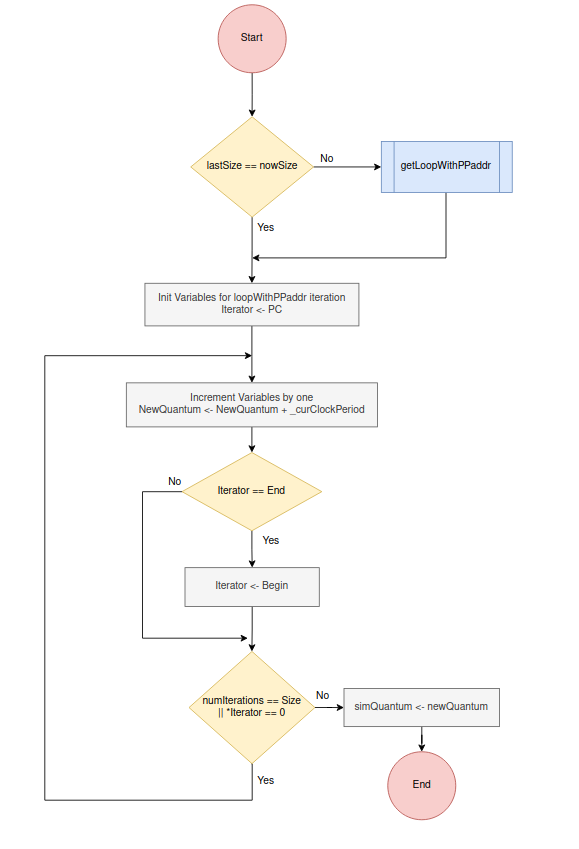
\includegraphics[width=0.6\linewidth]{Images/Repetition_flowchart_quantum.png}
 	\caption{Quantum calculation flowchart}
	 \label{fig_Repetition_flowchart_quantum}
\end{figure}

To calculate the quantum, the last tasks uses a iteration technique, as shown in detail in the \autoref{fig_Repetition_flowchart_quantum}. The iterator starts where the \gls{pc} is, and pursues the loop until it either finds a PPaddr, or reaches the starting point. The quantum starts with the minimum value, which is the clock period, and increments that value in each iteration done. 

\subsection{Results}

\autoref{fig:results_ADAINCPCREP} exhibits the results of the executed benchmarks with the previous (A-I-P) and new (REP) configurations. 

\begin{figure}[H]
\centering
\begin{subfigure}{\textwidth}
    \centering
    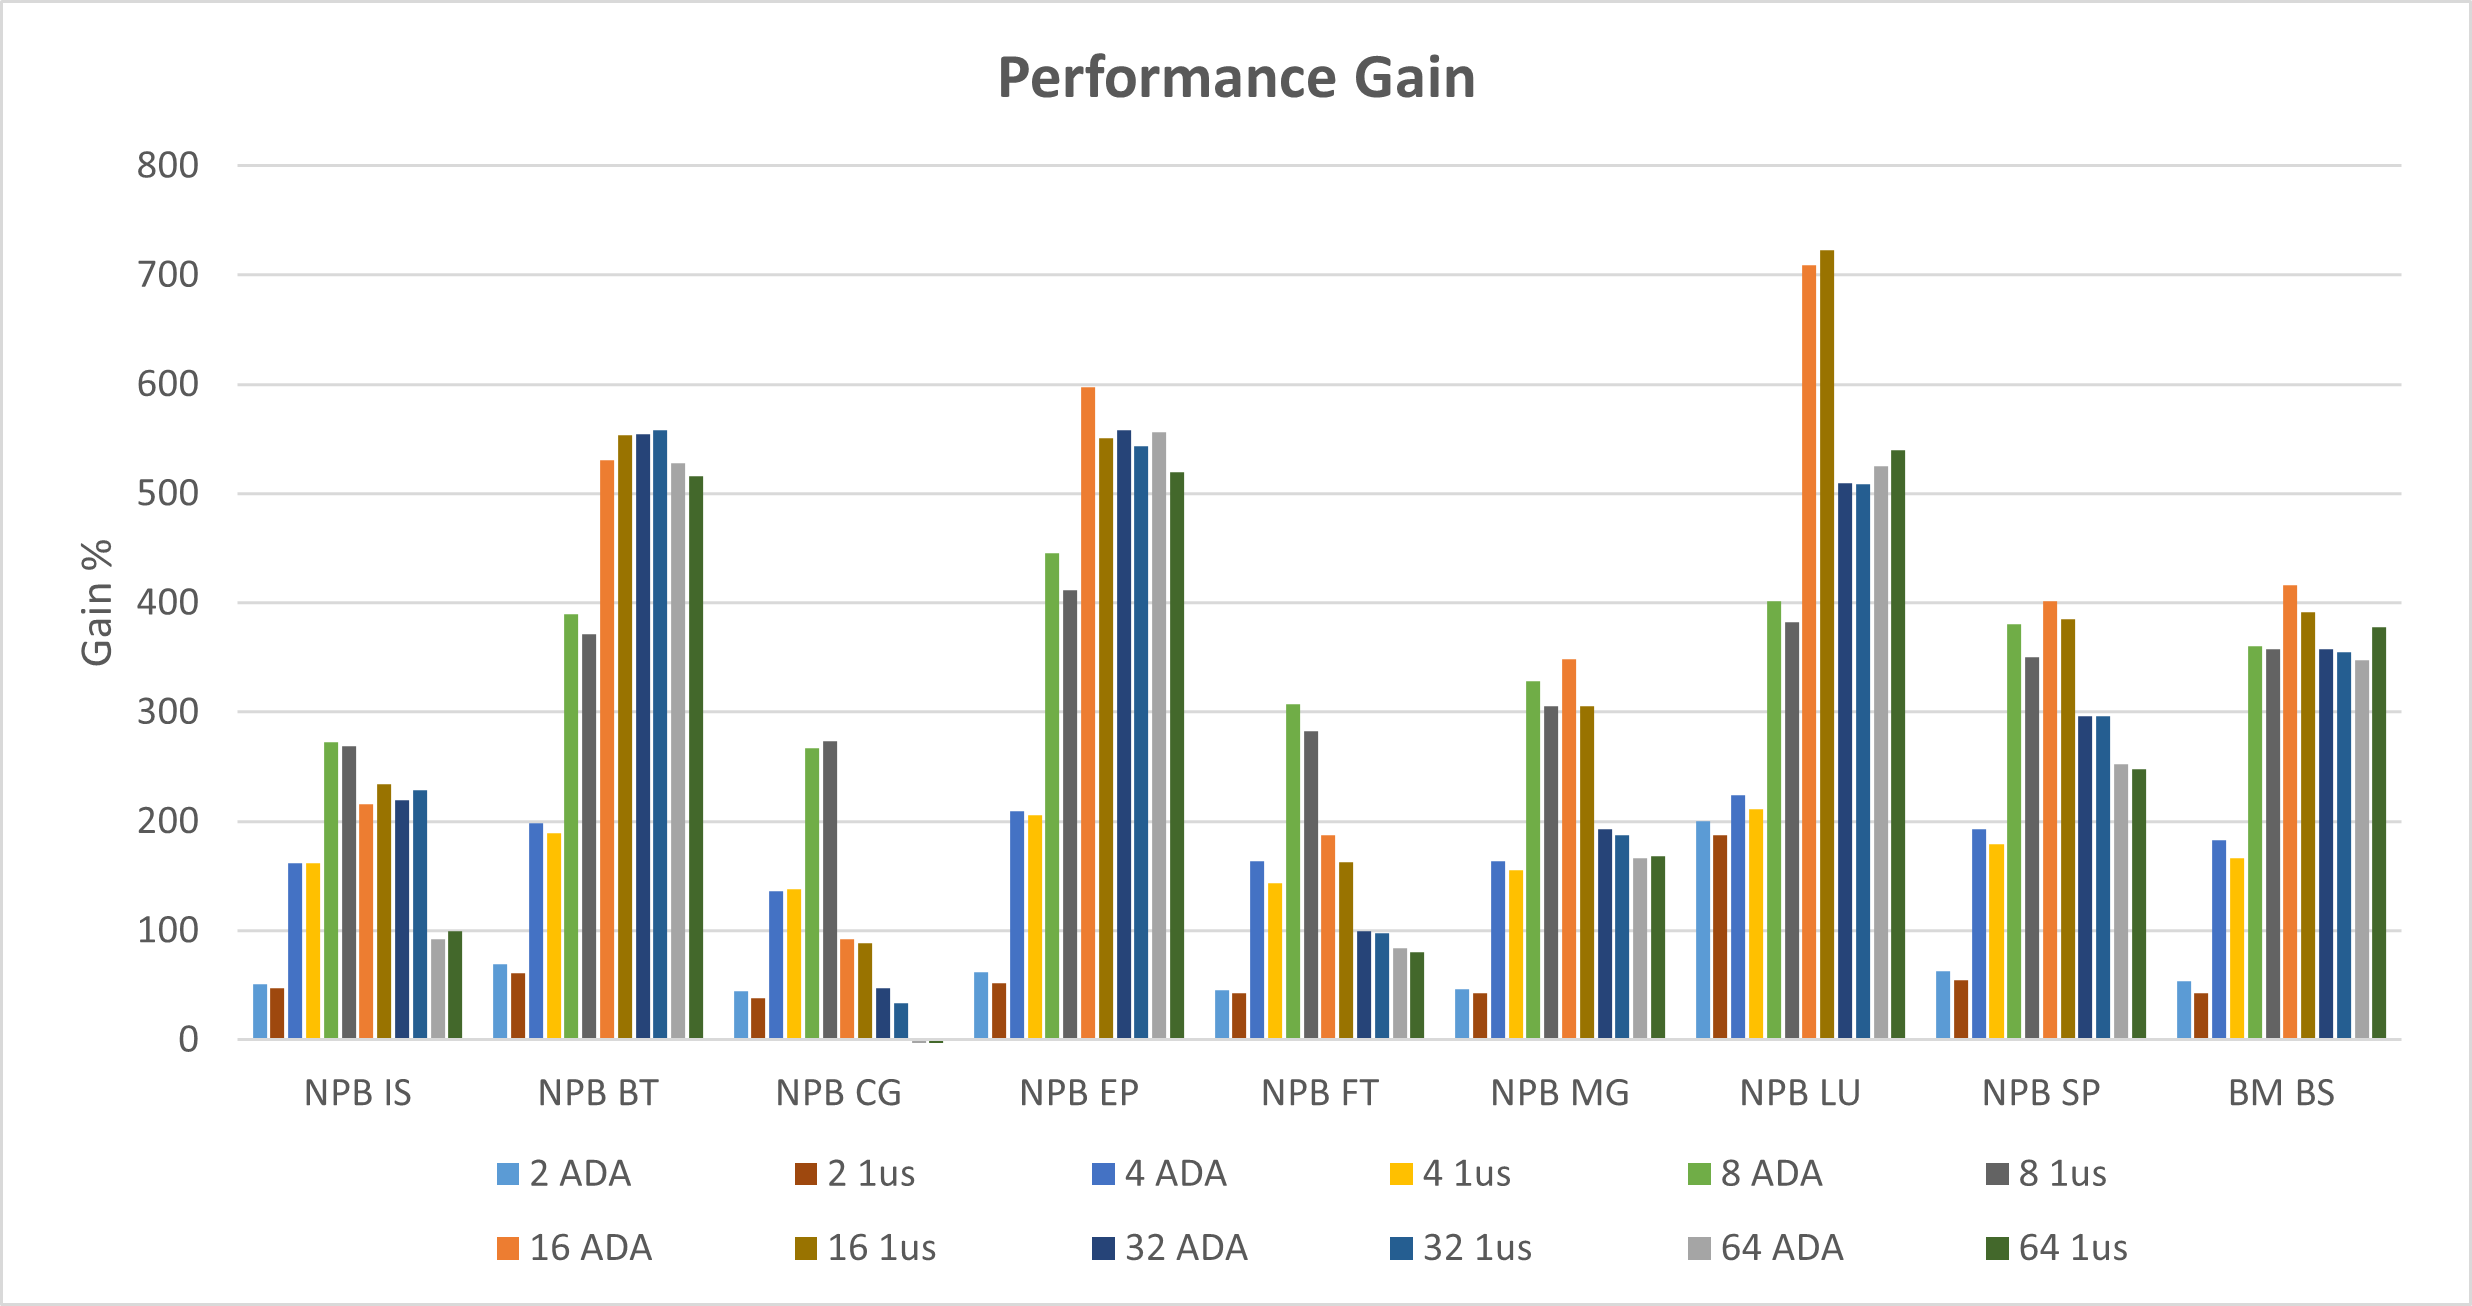
\includegraphics[width=0.75\textwidth]{Images/Performance_ADA.png}
    \caption{ Performance gain}
    \label{fig:Performance_ADAINCPCREP}
\end{subfigure}
\begin{subfigure}{\textwidth}
    \centering
    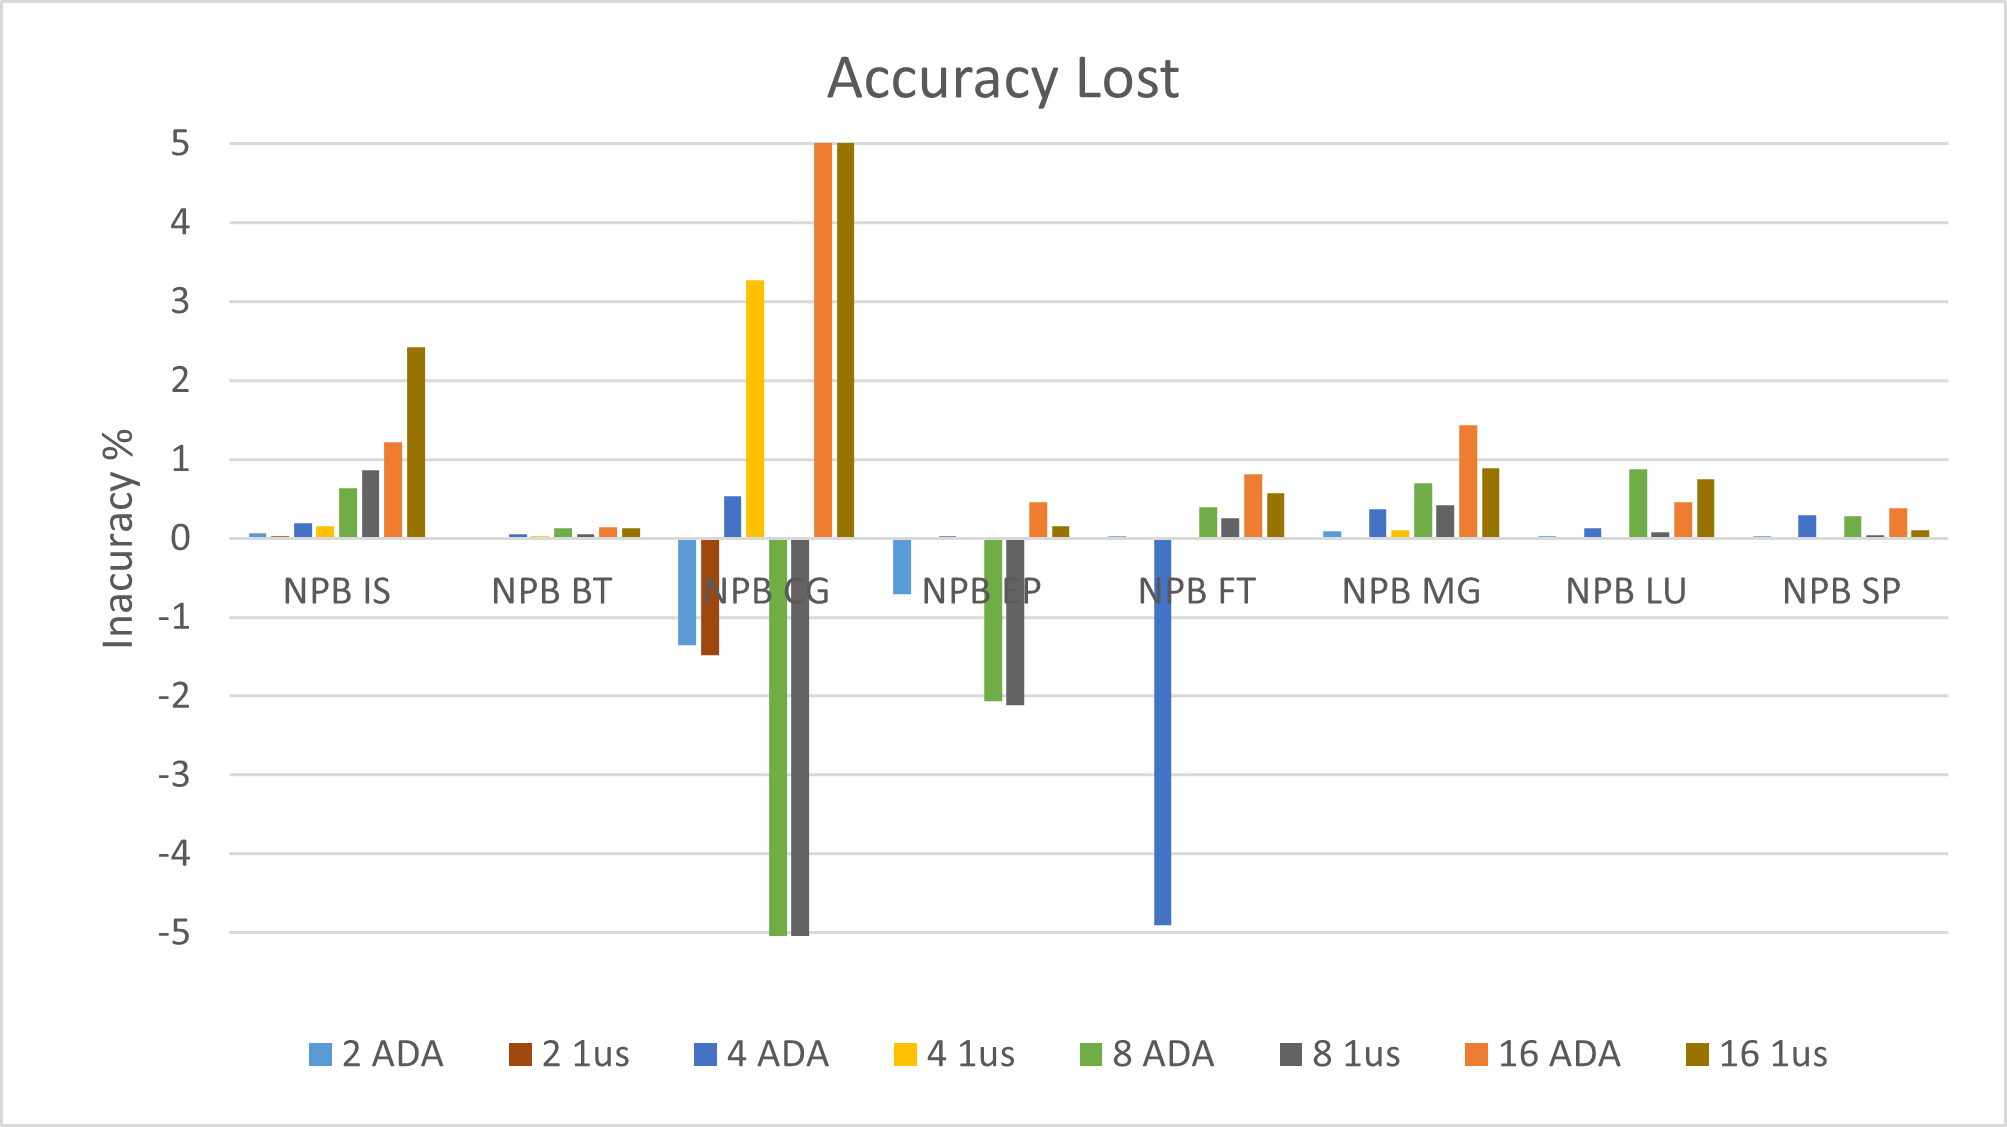
\includegraphics[width=0.75\textwidth]{Images/Accuracy_ADA.png}
    \caption{ Accuracy lost}
    \label{fig:Accuracy_ADAINCPCREP}
\end{subfigure}
\begin{subfigure}{\textwidth}
    \centering
    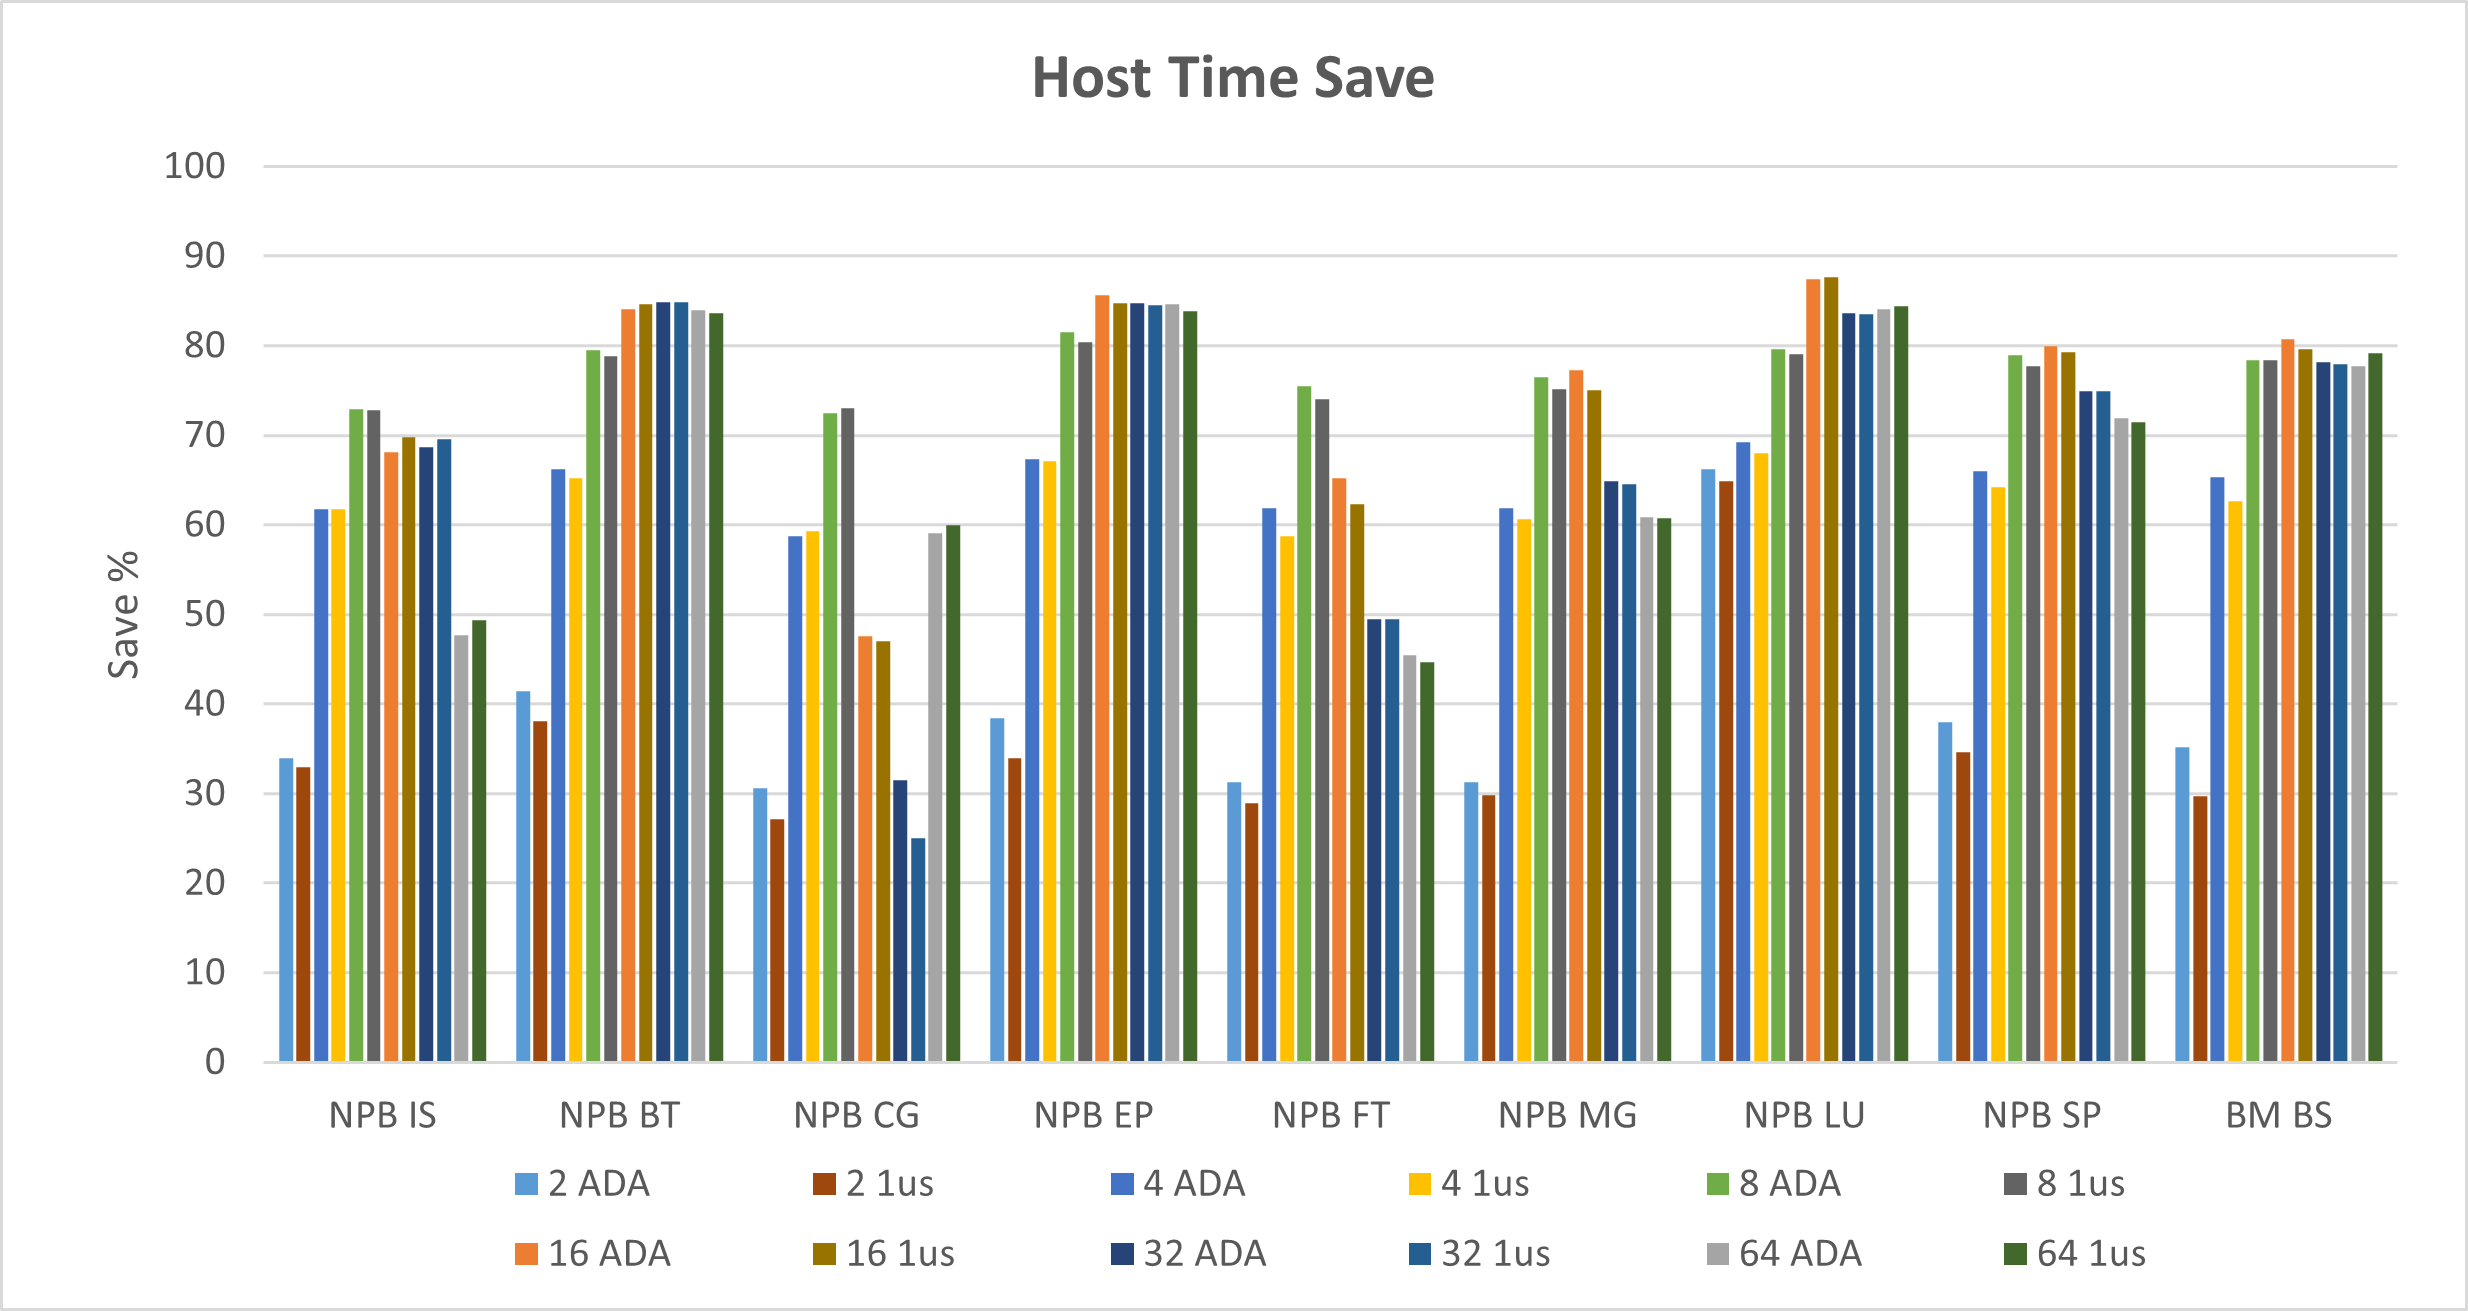
\includegraphics[width=0.75\textwidth]{Images/Host_ADA.png}
    \caption{ Host time save}
    \label{fig:Host_ADAINCPCREP}
\end{subfigure}
        
\caption{Repetitions algorithm results}
\label{fig:results_ADAINCPCREP}
\end{figure}



%Usar os resultados que já tenho, Verificar se está tudo

%COnclusão é que a performance e muito sacrificada

%O caso do CG e caso unico, explicar porque com prints que tenho guardadas
%Falar da natureza do CG algorithm

\section{Final Algorithm}

After the development and testing of all aforementioned algorithms, it was determined the better algorithm is the combination of the ADALINE, the dynamic increment, and the \gls{pc} analyses. The results show they complement each other, providing a great trade-off between performance and accuracy. The repetition algorithm was not integrated into the final solution due to its weak performance and accuracy gain. 

The synchronization process represented in the \autoref{fig_GlobalSyncEventStatic} can now be redefined to integrate the dynamic approach, as illustrated in the following flowchart. The static version was not removed because if there is a-priory information about the benchmark, the best quantum can be calculated before simulating. One example is a network application, where the communications delays are well-defined. If the quantum is set with the smaller delay, a perfect accuracy can be achieved \cite{dist-gem5}. 

\begin{figure}[H]
	\centering
 	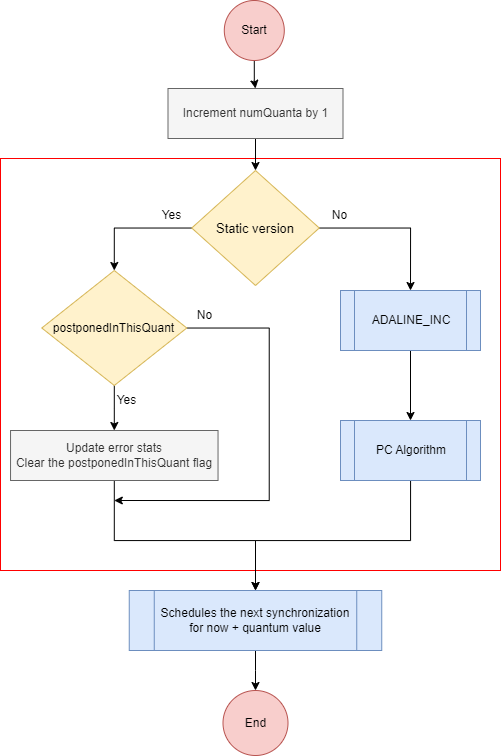
\includegraphics[width=0.5\linewidth]{Images/NewGlobalSyncEventStatic.png}
 	\caption{New quantum definition in the synchronization process}
	\label{fig_NewGlobalSyncEventStatic}
\end{figure}

\subsection{Results}

%Comparação com o 1us e o final

%Talvez falar sobre a media de quantum e quanto mais aumento com o modo dinamico















% \subsection{CPU model}

% To understand how can the prediction be made, it is important to understand the \gls{cpu} model in use. At the moment, par-gem5 \cite{pargem5} is restricted to the AtomicSimpleCPU model, which means is simpler and faster than the other versions. Nevertheless, the accuracy is sacrificed, because there is no verification, as presented in the \autoref{fig_AtomicMode}. The following image presents in detail its execution process.

% \begin{figure}[H]
% 	\centering
%  	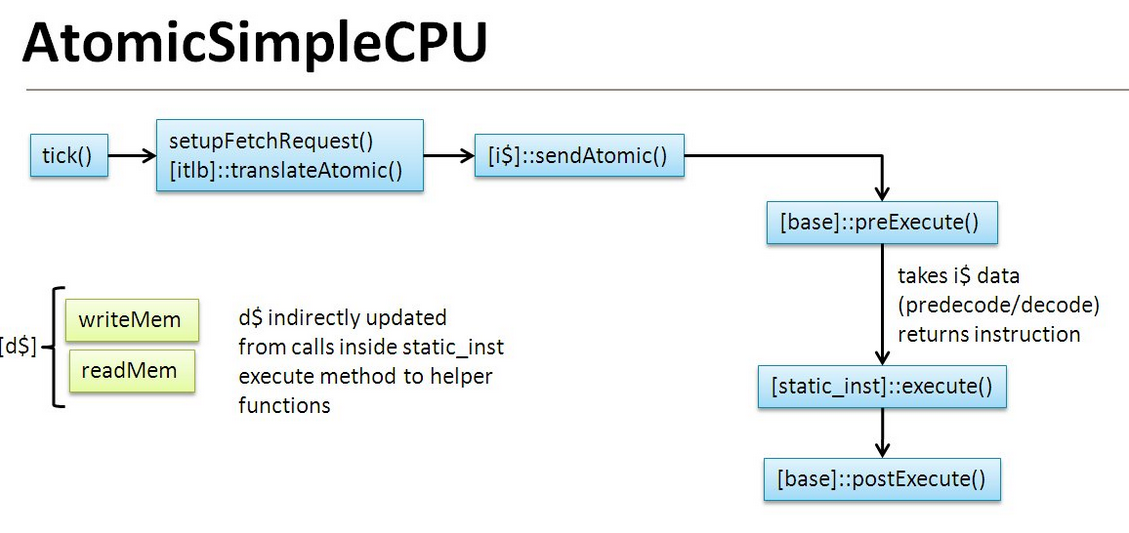
\includegraphics[width=0.7\linewidth]{Images/AtomicSimpleCPU.png}
%  	\caption{AtomicSimpleCPU execution process}
% 	 \label{fig_AtomicSimpleCPU}
% \end{figure}

% The tick event is responsible for stimulating the simulation

% %figure do atomic e explaicar onde deve de ser aplicado a deteçao.


